\documentclass[lettersize,journal]{IEEEtran}

% ── Core math ───────────────────────────
\usepackage{amsmath,amsfonts,amssymb}
\usepackage{amsthm}
\usepackage{bm}
\usepackage{mathtools}

% ── Theorem environments ──────────────────────────────────────────
\newtheorem{theorem}{Theorem}
\newtheorem{lemma}{Lemma}
\newtheorem{proposition}{Proposition}
\theoremstyle{definition}
\newtheorem{definition}{Definition}
\theoremstyle{plain}
\usepackage{subcaption}
\captionsetup{compatibility=false,figurename=Figure,tablename=Table}
% ── Algorithms ──────────────────────────
\usepackage{algorithm}
\usepackage{algpseudocode}

% ── Tables ──────────────────────────────
\usepackage{array}
\usepackage{booktabs}
\usepackage{tabularx}
\usepackage{multirow}
\usepackage{float}
% ── Figures ──────────────────────────────────────────

\usepackage{graphicx}
% figures/ lives at the repo root; this resolves whether pdflatex is run from
% the repo root or from paper/
\graphicspath{{./}{../}}
\usepackage{stfloats}
\usepackage[utf8]{inputenc}
\usepackage{textcomp}
\usepackage{url}
\usepackage{verbatim}
\usepackage{pifont}
\newcommand{\cmark}{\ding{51}}
\newcommand{\xmark}{\ding{55}}
\usepackage{bbm}
\usepackage{enumitem}
\usepackage{balance}
\usepackage{comment}
\usepackage[dvipsnames]{xcolor}
\usepackage[switch]{lineno}
\usepackage{cite}
\usepackage[colorlinks=true,
            linkcolor=blue,
            citecolor=blue,
            urlcolor=blue]{hyperref}

\DeclareMathOperator*{\argmin}{argmin}
\DeclarePairedDelimiter{\nint}\lfloor\rceil
\DeclarePairedDelimiter{\abs}\lvert\rvert


\newcommand{\best}[1]{\textbf{#1}}
\newcommand{\up}{$\uparrow$}
\newcommand{\down}{$\downarrow$}
\newcommand{\nd}{\textemdash}            % not defined / not applicable

\usepackage{booktabs}
\usepackage[table]{xcolor}
\usepackage{tikz}
\usepackage{xcolor}

\newcommand{\hmark}{%
  
\begin{tikzpicture}[scale=0.11, baseline=-0.6ex]
    \fill[orange] (0,0) circle (1);
    \fill[white] (0,0) -- (90:1.05) arc (90:-90:1.05) -- cycle;
  \end{tikzpicture}%
}


% (figure-placeholder macro removed: the manuscript contains no placeholders)


\renewcommand{\topfraction}{0.9}
\renewcommand{\bottomfraction}{0.8}
\renewcommand{\textfraction}{0.07}
\renewcommand{\floatpagefraction}{0.7}
\renewcommand{\dbltopfraction}{0.9}
\renewcommand{\dblfloatpagefraction}{0.7}
\setcounter{topnumber}{3}
\setcounter{bottomnumber}{2}
\setcounter{totalnumber}{5}
\setcounter{dbltopnumber}{3}

\hyphenation{op-tical net-works semi-conduc-tor IEEE-Xplore trans-form-er}

% =============================================================================
\begin{document}
% =============================================================================

\title{Toward One Trustworthy Explanation for Any Vision Transformer: Conservation-Valid Attribution via Attention Primitives}

\author{Nishankar~Sathiyamohan,~\IEEEmembership{Student~Member,~IEEE}%
  \thanks{Nishankar Sathiyamohan is a Lecturer with the Department of Computer
  Engineering, University of Peradeniya, Peradeniya 20400, Sri Lanka
  (e-mail: e17230@eng.pdn.ac.lk).}%
  \thanks{Manuscript submitted \today.}}

\markboth{IEEE Transactions on Image Processing,~Vol.~XX,~No.~X,~2026}%
         {Sathiyamohan: Toward One Trustworthy Explanation for Any Vision Transformer via Conservation-Valid Attribution}

\maketitle

% =============================================================================
\begin{abstract}
Vision Transformer (ViT) design has fragmented. Each new backbone recombines convolutional stems, windowed, linear, or multi-axis attention, patch merging, and spatial reduction, and each recombination invalidates a different attribution assumption: Grad-CAM needs a terminal spatial feature map, attention rollout needs global softmax attention, and layer-wise relevance propagation (LRP) needs a hand-derived rule per module type. To the best of our knowledge, no current method is both defined and trustworthy across this space. We demonstrate that this architectural space is structurally less complex than its variety suggests. The attention and resolution-reduction operators of current ViTs compose four types of operation: linear maps, bilinear mixing, normalization or gating, and reindexing. Each admits one relevance rule that conserves. The resulting method, HiLRP, covers a new backbone by construction rather than by derivation, and its map is a decomposition of the prediction rather than a heuristic. We prove conservation and conditional equivariance and verify both to machine precision. Benchmarking 14 attribution methods across 10 architectures, we find that no prior method is reliable across ViT families and that Faithfulness Correlation is uninformative on backbones robust to spatial masking. HiLRP alone stays conservation-valid on windowed, spatial-reduction, multi-axis, and linear-attention models, where naive extensions zero or inflate relevance, and it localizes where class activation mapping fails (0.97 against 0.55 Pointing on EfficientViT). The same backward pass yields stage-localized maps, attributes label-free self-supervised objectives, and explains CLIP image-text similarity with no new rule.
\end{abstract}

\begin{IEEEkeywords}
Explainable artificial intelligence, Vision Transformers, Hierarchical LRP, Relevance Propagation, Faithfulness, Localization, Shapley Agreement.
\end{IEEEkeywords}

% ================================================
\section{Introduction}
\label{sec:introduction}
\IEEEPARstart{V}{ision} transformers now underpin image analysis in domains where
a prediction on its own is not sufficient. In applications such as medical
imaging, remote sensing, and industrial inspection, the evidence supporting a
decision must be recoverable from the model, both to identify reliance on
spurious correlations and to document the basis of a decision before it is
acted upon. Post-hoc attribution methods address this requirement by assigning
each input pixel a score intended to express its contribution to the output.
Their usefulness rests on two conditions that are simple to state and, as this
paper shows, difficult to satisfy simultaneously: the method must be defined on
the architecture under analysis, and the scores it returns must carry a defined
meaning.

Neither condition is secure, because the architecture these methods were
designed around has since diversified. The Vision Transformer
(ViT)~\cite{dosovitskiy2021vit} began as a single design in which a fixed grid
of tokens is mixed by global self-attention. Current backbones retain the
transformer block but modify the operations surrounding it along three axes.
Attention is localized or linearized, through shifted local
windows~\cite{liu2021swin}, spatial reduction of the key and value
grid~\cite{wang2021pvt}, linear cross-covariance
products~\cite{cai2023efficientvit}, and multi-axis
schemes~\cite{tu2022maxvit}. Spatial resolution is reduced between stages by
token merging and strided projection. Convolutional and transformer stages are
interleaved in hybrid designs~\cite{mehta2022mobilevitv2}. Architectures of this
kind, together with DeiT~\cite{touvron2021deit}, BEiT~\cite{bao2022beit}, and
ConvNeXt~\cite{liu2022convnext}, appeared within roughly three years of one
another, each assembled for a particular domain or hardware budget from a small
inventory of components in a new arrangement. Attribution methods were not
revised at the same rate, and each retains an assumption that some current
backbone no longer satisfies.

\begin{figure}[!tbp]
  \centering
  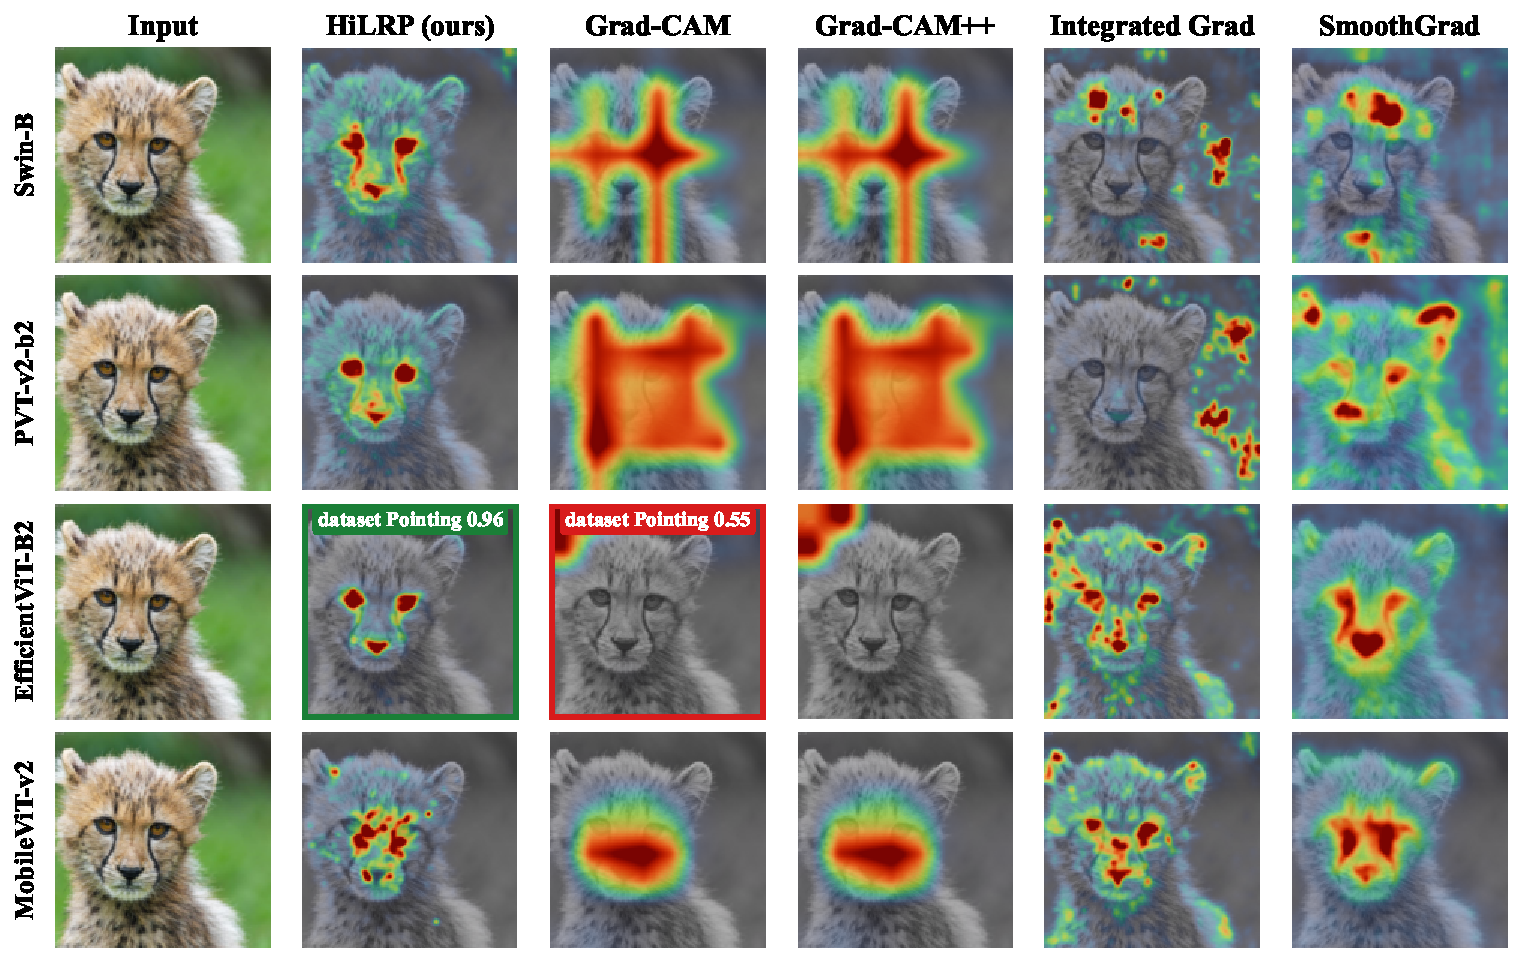
\includegraphics[width=\linewidth]{figures/bench/arch_method_comparison}
  \caption{Attribution maps over the desaturated input, one row per architecture. Grad-CAM and Grad-CAM++ remain coherent on Swin, PVT, and MobileViT but lose the object on EfficientViT-B2 (highlighted), whose linear attention lacks a terminal spatial feature map. HiLRP consistently focuses on the eyes and facial markings. 
  Scores are dataset-level Pointing values.}
  \label{fig:arch-comparison}
\end{figure}

This architectural divergence degrades attribution reliability in a manner that
is both measurable and specific to the method and backbone involved.
Figure~\ref{fig:arch-comparison} applies one set of attribution methods to a
single image across four backbones, so that only the architecture varies.
Grad-CAM~\cite{selvaraju2017gradcam} produces a coherent response on three of
them and a near-uniform response on EfficientViT, whose linear attention leaves
no terminal spatial feature map for class activation mapping (CAM) to weight.
The same pattern holds across the 10-architecture benchmark of
Sec.~\ref{sec:baseline-landscape}. Under the Pointing
Game~\cite{zhang2018pointing}, which records whether the highest-valued pixel of
an attribution falls inside the annotated object, Grad-CAM scores $1.00$ on four
backbones and $0.55$ on EfficientViT-B2, below the $0.61$ obtained by placing a
point at random. Attention Rollout~\cite{abnar2020rollout} is undefined on any
windowed or hierarchical model, and classic layer-wise relevance propagation
(LRP)~\cite{bach2015lrp} does not execute on modern transformer implementations.
These outcomes are not attributable to parameter selection. Each method depends
on a structural property that the backbone no longer provides.

The preceding cases are \emph{execution failures}: the method either cannot be
applied to the architecture or returns a map that is evidently degenerate. A
second class of failure preserves the appearance of a valid explanation while
eliminating its theoretical basis, namely the loss of the conservation guarantee
on which the method's interpretation depends.
AttnLRP~\cite{achtibat2024attnlrp} supplies propagation rules for the operations
inside a transformer block and conserves relevance through a flat transformer.
To the best of our knowledge, no corresponding rules have been reported for the
operations that make a backbone hierarchical. Applying the framework to such a
backbone therefore requires relying on unmodified gradients for the unsupported
layers, and the scale-invariant normalizations among those layers drive the
propagated relevance towards zero. Across five hierarchical backbones the
resulting relevance is inflated more than threefold on one and reduced to
exactly zero at depth on the remaining four
(Sec.~\ref{sec:conservation-validity}), while the maps continue to localize
well. A map whose values sum to zero retains a maximum and therefore still
satisfies a localization criterion, so a conservation-valid attribution and a
degenerate one are indistinguishable under the criteria commonly reported.

The two classes of failure together define two requirements. An attribution
method must be \emph{defined} on the architecture under analysis, and the values
it returns must \emph{decompose} the prediction rather than rank pixels by an
unconstrained score. Existing work satisfies one requirement or the other.
Gradient and perturbation methods execute on any architecture but establish no
conservation property, so the quantity their values sum to is unconstrained.
LRP~\cite{bach2015lrp} and its transformer
descendants~\cite{chefer2021transformer,achtibat2024attnlrp} do constrain that
quantity, through layer-wise conservation, but only for isotropic transformers,
and their extension has so far required a separately derived rule for each new
module type, a cost that grows with the number of architectures rather than
diminishing as the design space expands.

Rather than deriving a separate propagation rule for each new architectural
module, this work shows that the operators in question decompose into a small
set of primitive computational types. The architectures above differ in how
their operations are \emph{arranged}, not in which operations they \emph{use}.
Every attention
mechanism and every resolution-reduction operator in this class of models is
assembled from four types of computation: linear maps, such as the query, key,
value, and output projections; bilinear products, in which both factors depend
on the input; normalizations and gates, such as the softmax and LayerNorm; and
reindexings, such as reshaping, window partitioning, and cyclic shifting.
Windowed attention and spatial-reduction attention, for instance, contain the
same four types arranged in a different order and over a different sparsity
pattern. Each type admits a single relevance rule that conserves, and a
composition of conserving operations is itself conserving
(Proposition~\ref{prop:closure}). A rule set covering the four types therefore
covers any architecture assembled from them, in any arrangement, with no further
derivation.

Hierarchical LRP (HiLRP) is the attribution method built on this decomposition.
Supporting a backbone requires only assigning each of its modules to one of the
four types, after which the rules and the conservation proof are inherited.
Patch merging, shifted-window partitioning, and spatial reduction, the
operations that motivated this work, are not the framework but one instance of
it, since all three are the same linear projection applied to a concatenated
token neighborhood. The resulting guarantee is not unconditional: an
architecture built on a fundamentally distinct mixing operation, such as the selective
scan of a state-space model, requires one additional rule, which the
construction admits but which we do not derive here.

Establishing these claims requires evaluation criteria that can separate a valid
attribution from an invalid one, and the criteria in standard use cannot.
Perturbation-based fidelity measures assume that masking an important region
changes the prediction, an assumption modern ViTs violate, and across our
benchmark the resulting scores are statistically indistinguishable from noise.
Localization measures fail differently: on datasets of large centered objects, a
fixed Gaussian blob that never examines the image saturates the Pointing Game
and outscores most attribution methods on average precision. We therefore
evaluate on three axes that a model-free map cannot win, namely conservation
validity, agreement with sampled Shapley values over image segments, and
relevance mass inside the object measured against the area a uniform map would
already cover (Sec.~\ref{sec:energy-localization}).

This paper makes four contributions.

\begin{itemize}[leftmargin=1.2em]
  \item \textbf{Attribution from four primitives.} We decompose the attention and resolution-reduction operators of current ViTs into four operation types, each with one conserving relevance rule, so coverage of a backbone is a matter of construction rather than derivation. Conservation and conditional equivariance are proved and verified to machine precision. We further show that patch merging, shifted-window partitioning, and spatial reduction are three instances of a single algebraic form, namely a learned linear projection applied to a concatenated neighborhood of tokens, $W\phi(\mathrm{concat}(\cdot))$. One rule and one proof consequently cover all three operations, in place of a separate derivation for each.

  \item \textbf{Compositional coverage of the attention taxonomy.} We verify the decomposition for self-, cross-, and co-attention, together with windowed, linear, spatial-reduction, multi-axis, channel, dilated, and deformable attention, realize eight on pretrained backbones, and attribute a cross-modal scalar on CLIP without adding a rule. Because conservation composes, a mechanism outside the four costs one added rule and leaves the existing rules intact, so coverage grows by extension rather than by rederivation.

  \item \textbf{Conservation validity where prior work is degenerate.} On the windowed, spatial-reduction, multi-axis, and linear-attention families, the naive extension of attention-aware LRP zeroes or inflates relevance while still scoring well on localization, and classic LRP does not run. HiLRP keeps a bounded, non-degenerate decomposition on all five. Globally-normalized convolution hybrids such as MobileViT fall outside the present primitive set and are treated as a designated extension (Sec.~\ref{sec:limitations}).

  \item \textbf{A cross-architecture benchmark and an evaluation protocol that survives it.} Over 10 architectures and 14 methods we show that no prior attribution is reliable across ViT families, and that Faithfulness Correlation (FC) is statistically indistinguishable from noise in all $118$ model-method cells on which it is defined. Under conservation validity and Shapley agreement, HiLRP is the only method that holds on every family, including the linear-attention backbones where Grad-CAM fails in both localization ($0.97$ against $0.55$) and Shapley agreement ($0.417$ against $0.077$).
\end{itemize}

The rest of the paper is organized as follows. Section~\ref{sec:related} reviews attribution methods, conservation-based propagation, and existing cross-architecture evaluations. Section~\ref{sec:methodology} develops HiLRP: the unifying form of resolution reduction, the four primitives and their rules, the conservation and equivariance guarantees, the label-free extension, and the implementation. Section~\ref{sec:setup} states the experimental protocol and why the standard fidelity metric is replaced. Section~\ref{sec:results} reports the benchmark, localization, conservation validity, Shapley agreement, stage-localized and multi-modal attribution, the pretraining study, and the ablations. Section~\ref{sec:limitations} states the limitations and Section~\ref{sec:conclusion} concludes.

% =============================================================================
\section{Related Work}
\label{sec:related}

\subsection{Attribution Methods}
Attribution methods fall into four broad families: gradient-based, attention-native, perturbation-based, 
and propagation-based. Gradient methods, including
Saliency~\cite{simonyan2014saliency}, Integrated
Gradients~\cite{sundararajan2017ig}, Input$\times$Gradient~\cite{shrikumar2017deeplift}, 
SmoothGrad, and VarGrad~\cite{smilkov2017smoothgrad}, differentiate the class logit with 
respect to the input. CAM methods, namely Grad-CAM~\cite{selvaraju2017gradcam} and
Grad-CAM++~\cite{chattopadhay2018gradcampp}, weight intermediate feature maps by the gradient signal; 
applying them to a ViT requires reshaping the token sequence back into a spatial grid. Attention-native methods 
such as Attention Rollout~\cite{abnar2020rollout} and the relevance-propagation attribution of Chefer et~al.~\cite{chefer2021transformer, bach2015lrp} 
exploit the transformer's own attention maps and have no convolutional counterpart. Perturbation methods, 
including Occlusion~\cite{zeiler2014occlusion}, RISE~\cite{petsiuk2018rise}, LIME~\cite{ribeiro2016lime}, and GradientSHAP~\cite{lundberg2017shap}, 
probe the model by masking or sampling the input; they are model agnostic but computationally costly. The present benchmark evaluates representatives 
of all four families (Table~\ref{tab:taxonomy}). Each family rests on an architectural assumption that a sufficiently different backbone can invalidate: 
CAM assumes a terminal spatial feature map, attention-native methods assume explicit softmax attention matrices, and gradient methods assume smoothly 
behaved input gradients.


\begin{table}[!tbp]
  \centering
  \caption{\textbf{Attribution families and their architectural assumptions.}
  Rows show method families and their required assumptions; columns show backbone
  families. A check indicates that the assumption holds, a half-disk indicates
  degraded or unstable behavior, and a cross indicates that the method is
  undefined or fails to run. HiLRP avoids these architecture-specific
  assumptions by operating on four conservation-preserving primitives.}
  \label{tab:taxonomy}
  \setlength{\tabcolsep}{1.8pt}
  \scriptsize
  \begin{tabular}{@{}llccccccc@{}}
    \toprule
    \textbf{Family} & \textbf{Assumption}
    & \textbf{CNN} & \textbf{ViT} & \textbf{Swin}
    & \textbf{PVT} & \textbf{MaxV} & \textbf{MobV} & \textbf{EffV} \\
    \midrule
    Gradient
      & smooth gradients
      & \cmark & \hmark & \hmark & \hmark & \hmark & \hmark & \hmark \\
    CAM
      & spatial feature map
      & \cmark & \hmark & \cmark & \cmark & \cmark & \cmark & \xmark \\
    Attention
      & softmax $+$ \textsc{cls}
      & \xmark & \cmark & \xmark & \xmark & \xmark & \xmark & \xmark \\
    Perturbation
      & output access
      & \cmark & \cmark & \cmark & \cmark & \cmark & \cmark & \cmark \\
    Classic LRP
      & module-specific rules
      & \cmark & \xmark & \xmark & \xmark & \xmark & \xmark & \xmark \\
    \midrule
    \rowcolor{green!10}
    \textbf{HiLRP (ours)}
      & four primitives
      & \cmark & \cmark & \cmark & \cmark & \cmark & \cmark & \cmark \\
    \bottomrule
  \end{tabular}
\end{table}

\subsection{Conservation-Based Attribution and the Hierarchical Gap}
\label{sec:related-lrp} 
LRP~\cite{bach2015lrp} is distinguished from the families above by a completeness property: relevance is conserved layer by layer, so the explanation is a decomposition of the prediction rather than a saliency heuristic. Chefer et~al.~\cite{chefer2021transformer} extended this framework to isotropic ViTs by combining relevance with attention gradients, and AttnLRP~\cite{achtibat2024attnlrp} derived block-internal rules that preserve conservation through a transformer's non-linear operations: a Taylor rule for the softmax, a uniform split for the bilinear matrix products, and an identity rule for LayerNorm. These methods conserve, but only for flat, all-to-all transformers. Neither of them defines a rule for the operations that make a modern ViT hierarchical or hybrid: patch merging, shifted-window partitioning, spatial reduction, convolutional stems, or the linear-attention denominator. Applied to such backbones, they either fail to execute when an unsupported layer is reached, or inadvertently violate conservation when a scale-invariant normalization drives the propagated relevance to zero (Sec.~\ref{sec:conservation-validity}). The conventional approach of manually deriving one rule per new module does not scale to the rapid proliferation of novel architectures. HiLRP instead reduces every such operation to a small set of conserving primitives, closing the gap by construction rather than by enumeration.

\subsection{Evaluating Explanations}
A ground truth for a correct attribution is rarely available, so evaluation relies on surrogate criteria. Faithfulness metrics perturb high-attribution regions and measure the resulting change in the model output~\cite{bhatt2020faithfulness,alvarez2018robustness,rong2022road}. Localization metrics compare attributions against object masks or boxes through the Pointing Game~\cite{zhang2018pointing}. Robustness metrics such as Max-Sensitivity~\cite{yeh2019sensitivity} measure stability under small input perturbations, complexity metrics~\cite{chalasani2020sparseness} quantify how concentrated an explanation is, and sanity checks~\cite{adebayo2018sanity} test whether an attribution depends on the model at all. Systematic reviews and benchmark studies~\cite{nauta2023anecdotal,bodria2023benchmarking} report that these criteria often disagree and that no single metric suffices, which motivates a multi-metric protocol. We adopt the \textsc{Quantus}~\cite{hedstrom2023quantus} library so that every metric is computed by a shared and validated implementation rather than through a separate custom implementation.

\subsection{Ground-Truth and Cross-Architecture Benchmarks}
Brandt et~al.~\cite{brandt2023precise} obtain an exact ground truth by hand-constructing a small CNN, and report that Integrated Gradients performs best overall and that methods are weak on negatively contributing pixels. Their study is confined to a $36\times36$ CNN evaluated solely on synthetic inputs. FunnyBirds~\cite{hesse2023funnybirds} and CLEVR-XAI~\cite{arras2022clevrxai} provide causal or synthetic ground truth, again primarily for CNNs, while systematic evaluations of attribution methods have to date concentrated on convolutional backbones~\cite{rao2022attribution}. Among proxy-based evaluations, \textsc{Quantus}~\cite{hedstrom2023quantus} and ROAD~\cite{rong2022road} scale to real models but provide no ground truth and can disagree. Recent work has examined the faithfulness of ViT explanations directly~\cite{wu2024faithfulness}, but on isotropic ViTs, and without examining whether a method remains \emph{defined and conservation-valid} as the backbone design changes. To the best of our knowledge, no prior study evaluates attribution across the breadth of modern hierarchical and hybrid ViT designs under a single fixed protocol while testing, on the same axis, whether the explanations conserve relevance at all. This combination constitutes the gap addressed in the present work.

\textbf{Concurrent and adjacent directions.} Transformer LRP was established for flat self-attention by AttnLRP~\cite{achtibat2024attnlrp}, upon which our block-internal rules are based; recent efforts extend attribution to hierarchical designs, but per-architecture rather than through a shared primitive decomposition. Two model families lie outside our current primitive set and represent logical extensions for future work. State-space vision models (Vision Mamba and related selective-scan backbones) mix tokens through a linear recurrence rather than a bilinear attention product, a fundamentally distinct mixing primitive that would require one additional conserving rule, which the framework is designed to admit. Generative diffusion backbones are a second such family. Explanation methods for diffusion models have received increasing attention, but those proposed to date are attention- and saliency-based rather than conservation-based: Park et~al.~\cite{park2024explaindiffusion} explain the denoising trajectory through visual analysis of cross-attention across time steps, and ConceptAttention~\cite{helbling2025conceptattention} derives saliency maps from the attention layers of a diffusion transformer to localize textual concepts. Both produce a ranking over image regions; neither establishes that the values returned decompose a scalar the model computes. Carrying the conservation premise to this family therefore requires two additions: a target scalar appropriate to a generative rather than a discriminative objective, and rules for any mixing operation the denoiser introduces beyond the four types treated here. We accordingly position HiLRP as the conservation-valid attributor for the current, attention-based ViT design space, and identify state-space mixing and generative denoising objectives as the two extensions the framework is designed to accommodate.

% =============================================================================
\section{Methodology: HiLRP}
\label{sec:methodology}

\subsection{Notation and the Conservation Constraint}
\label{sec:notation}
Let $x\in\mathbb{R}^{H\times W_{\mathrm{img}}\times 3}$ be the input image, $f$ the frozen network, $c$ the index of the class being explained, and $f_c(x)\in\mathbb{R}$ the corresponding output logit. Activations inside the network are written $a$, with subscripts giving spatial position and channel; the symbol $x$ is reserved for the input image throughout, and $y$ denotes the output of whichever operator is under discussion.

\emph{Relevance} denotes the quantity that LRP redistributes from the output of the network back towards its input. For an activation $a_j$, the scalar $R_j$ denotes the portion of the output logit $f_c(x)$ attributed to that activation. Propagation is initialized at the output with $R=f_c(x)$ and proceeds backward layer by layer, subject at every layer to the conservation constraint

\begin{equation}
\label{eq:conservation}
\sum_{j\,\in\,\text{layer }\ell} R_j \;=\; \sum_{i\,\in\,\text{layer }\ell+1} R_i
\;=\; f_c(x),
\end{equation}

where $\ell$ indexes depth. The condition in Eq.~\eqref{eq:conservation} distinguishes a relevance map from a saliency heuristic: it forces the attribution delivered at the input pixels to be a decomposition of $f_c(x)$, so the values carry the units of the prediction and sum to it. Standard LRP rules, including the $\epsilon$-rule and the $z^{+}$-rule, satisfy Eq.~\eqref{eq:conservation} for linear layers and convolutions. Remaining symbols are defined where they first appear.

For the three operations identified in Sec.~\ref{sec:related-lrp} as lacking a propagation rule, we
first show that all three are instances of a single algebraic form, so one rule and one proof cover
them, and then give the concrete rules, the conservation and equivariance guarantees, the
label-free extension, and the implementation.

HiLRP inherits the block-internal attention rules of AttnLRP~\cite{achtibat2024attnlrp} listed in
Sec.~\ref{sec:related-lrp}. The novel contributions introduced in this methodology are fourfold: the resolution-reduction rule that unifies patch merging, shifted 
windows, and spatial reduction as one coordinate-embedded linear map; the normalization-subclass 
guard that prevents scale-invariant norms from silently zeroing deep relevance; the 
conservation-preserving attention rule (CP-LRP, Sec.~\ref{sec:cp}) applied uniformly across families; and the 
four-primitive framework that makes coverage a matter of construction rather than per-architecture 
derivation.

\subsection{A Unifying View of Resolution Reduction}
\label{sec:unifying}
The diverse downsampling operators utilized across ViT variants can be mathematically reduced to a single formulation. Let $\mathcal{N}=\{a^{(1)},\dots,a^{(n)}\}$ be the ordered set of $n$ input tokens consumed by a single resolution-reduction step ($n{=}4$ for $2{\times}2$ patch merging, $n{=}k^2$ for a $k{\times}k$ strided kernel), with each token $a^{(i)}\in\mathbb{R}^{d_{\mathrm{in}}}$. Patch merging concatenates a $2{\times}2$ neighborhood and projects it; a strided patch-embedding convolution is a linear map on a pixel neighborhood; and the spatial reduction in PVT and EfficientViT is a strided convolution on the token grid. Each can be written as
\begin{equation}
\label{eq:unifying}
T(\mathcal{N}) = W\,\phi\!\left(\mathrm{concat}(a^{(1)},\dots,a^{(n)})\right) = y \in \mathbb{R}^{d_{\mathrm{out}}},
\end{equation}
where $\mathrm{concat}:(a^{(1)},\dots,a^{(n)})\mapsto [a^{(1)\top},\dots,a^{(n)\top}]^\top \in \mathbb{R}^{nd_{\mathrm{in}}}$ is a coordinate embedding (one input coordinate per output coordinate, exact by Lemma~\ref{lem:conservation}), $\phi:\mathbb{R}^{nd_{\mathrm{in}}}\to\mathbb{R}^{nd_{\mathrm{in}}}$ is a conservation-preserving normalization (identity or LayerNorm), and $W\in\mathbb{R}^{d_{\mathrm{out}}\times nd_{\mathrm{in}}}$ is the learned projection. The output $y$ is the single merged token produced from neighborhood $\mathcal{N}$. The form in Eq.~\eqref{eq:unifying} is therefore the operator through which HiLRP propagates relevance across a change of resolution. A single rule for this operator yields patch merging, strided patch embedding, and spatial reduction as corollaries, rendering the framework architecture-agnostic rather than a collection of per-model modifications. The cyclic shift and the window partition of the shifted-window mechanism are pure permutations of $\mathcal{N}$, which require no rule of their own: by Lemma~\ref{lem:conservation} a permutation conserves relevance exactly, and the Gradient$\times$Input backend propagates such an operation through native automatic differentiation.

\subsection{Attention as Four Conserving Primitives}
\label{sec:primitives}
The same reduction applies to attention itself, rendering HiLRP general rather than a collection
of per-architecture rules. Every attention mechanism we survey, from global softmax to linear 
cross-covariance, is a composition of four operation classes. Each is defined by its algebraic
form rather than its specific module implementation, as the mathematical form dictates the
applicable propagation rule.

\begin{definition}[Linear map]
\label{def:linear}
An operation $y_i=\sum_j w_{ij}a_j + b_i$ with weights independent of the
activations. Instances: the $Q$, $K$, $V$, and output projections, poolings,
kernel feature maps, rotary and relative-position embeddings, and the
resolution-reduction map of Eq.~\eqref{eq:unifying}. Rule: the $\epsilon$/$\gamma$
rule of Eq.~\eqref{eq:gamma-rule}, which conserves by Lemma~\ref{lem:conservation}
up to the bias and stabilizer.
\end{definition}

\begin{definition}[Bilinear mixing]
\label{def:bilinear}
An operation $y=UV$ in which \emph{both} factors depend on the activations, so
the map is not linear in either alone. Instances: the matrix products $QK^\top$ and
$AV$, the linear-attention products, and deformable sampling at learned offsets.
Rule: a uniform split of relevance between the two factors, or, in the
conservation-preserving variant used throughout (Sec.~\ref{sec:cp}), the
treatment of one factor as fixed gating so that relevance flows through the other.
\end{definition}

\begin{definition}[Normalization and gating]
\label{def:norm}
An operation $y = a \odot g(a)$ or $y = a / d(a)$ whose second factor is a scalar
or per-group statistic computed from the activations themselves. Instances:
softmax, the linear-attention denominator, LayerNorm, and squeeze-excite or
sigmoid gates. Rule: detach the denominator or gate, making the operation locally
linear in the numerator, which conserves exactly in the detached variable.
\end{definition}

\begin{definition}[Reindexing]
\label{def:reindex}
An operation that moves activations without combining them, so its matrix has exactly one nonzero entry per output. Instances: head splitting and merging, window partitioning, cyclic shifting, dilation, grouping, and the concatenation of Eq.~\eqref{eq:unifying}. Rule: none is needed. By Lemma~\ref{lem:conservation} the ratio $z_{ij}/z_i$ is one, so relevance is copied without leak.
\end{definition}

\noindent Four rules are sufficient to cover an unbounded set of architectures because conservation is preserved under composition.

\begin{proposition}[Closure under composition]
\label{prop:closure}
Let $f = f_L \circ \cdots \circ f_1$ where each $f_\ell$ is one of
Definitions~\ref{def:linear}--\ref{def:reindex} and each satisfies
$\sum_j R^{(\ell)}_j = \sum_i R^{(\ell+1)}_i$. Then $f$ satisfies
Eq.~\eqref{eq:conservation} end to end.
\end{proposition}

\begin{proof}
Immediate by induction on $\ell$: the relevance entering layer $\ell$ equals that leaving layer $\ell+1$ by hypothesis, so the total is invariant along the composition and equals the seed $f_c(x)$.
\end{proof}

\noindent Proposition~\ref{prop:closure} converts a set of four rules into coverage of an entire architecture family. Fundamentally, attention comprises a linear map, followed by a bilinear mix, a normalization or gate, and an aggregation over some sparsity pattern. HiLRP conserves relevance through each of these stages, and therefore through their composition. Fig.~\ref{fig:attnlrp-propagation} traces this decomposition through one multi-head attention block, colouring each operation by the primitive it belongs to and marking where the relevance rule for that primitive applies.

\begin{figure*}[!t]
\centering
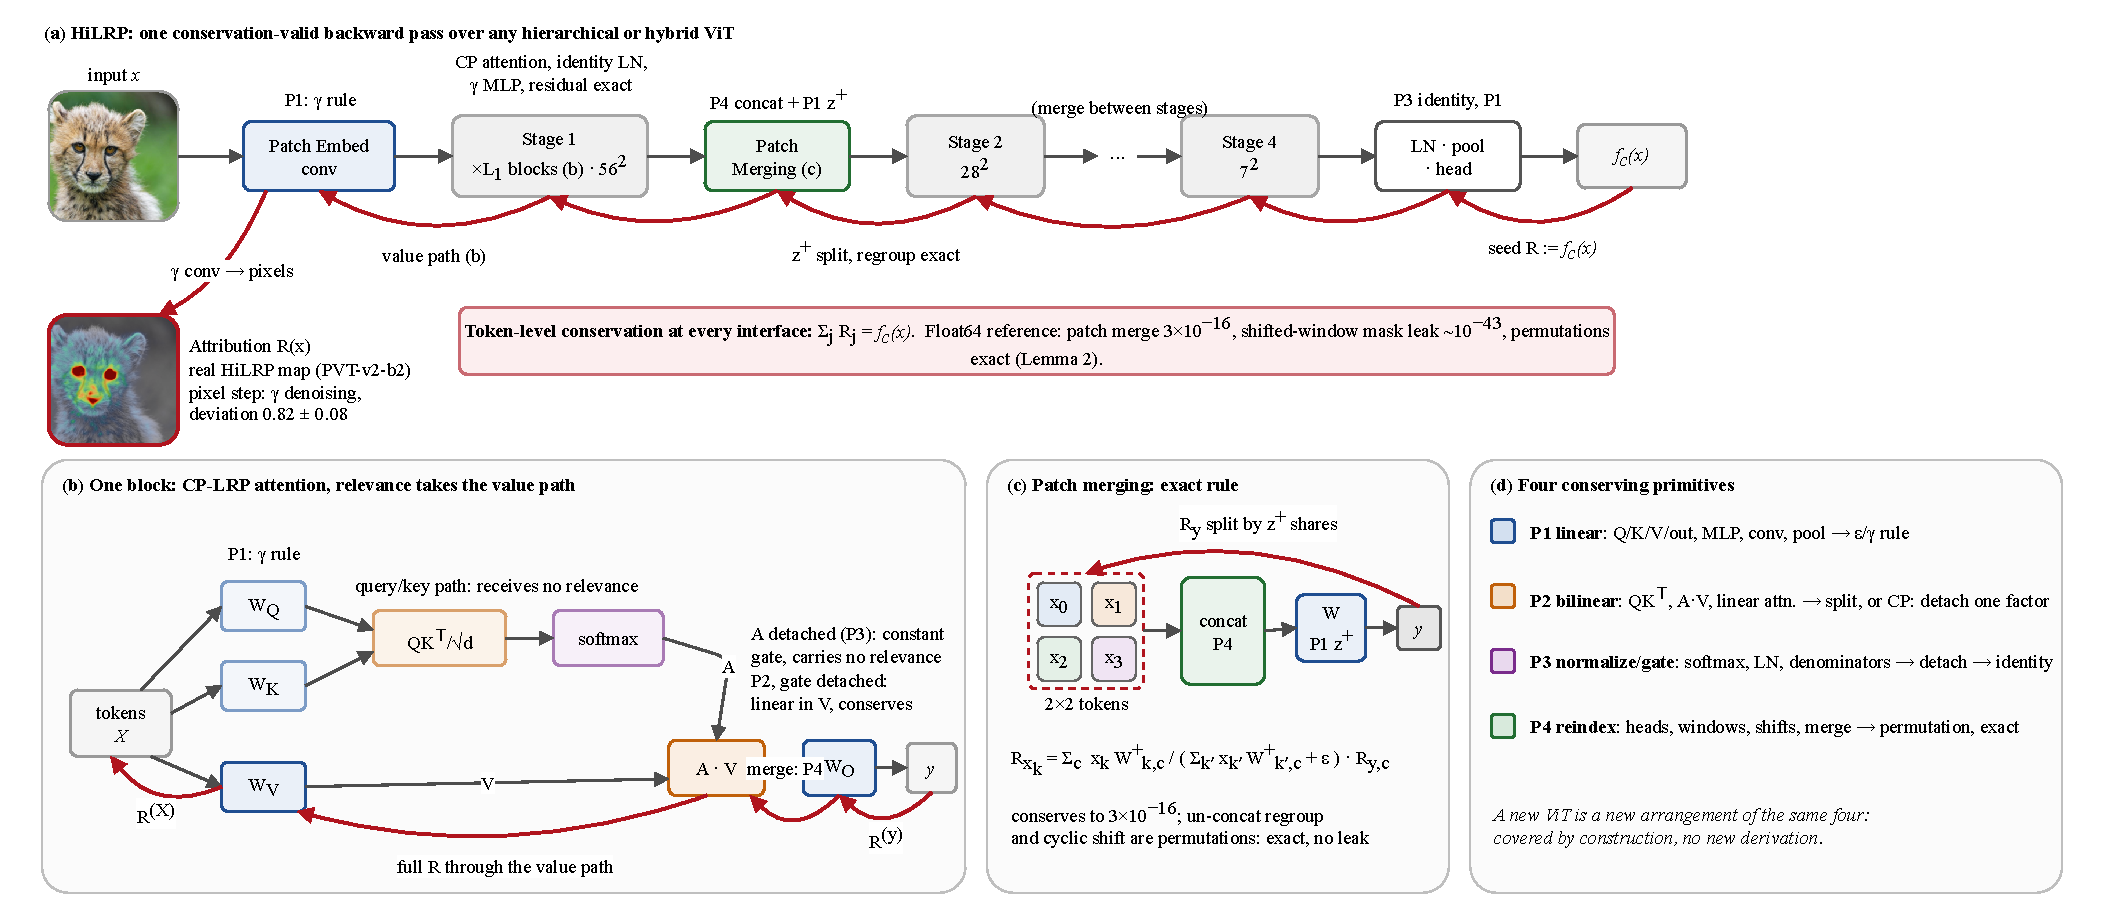
\includegraphics[width=\textwidth]{figures/hilrp/hilrp_pipeline.pdf}
\caption{\textbf{HiLRP overview.} Forward propagation in black, relevance in red.
(a) One backward pass over a hierarchical backbone.
(b) Attention block under CP-LRP: relevance follows the value path.
(c) Patch merging, the $z^{+}$ rule of Eq.~\eqref{eq:merge-rule}.
(d) The four primitives and their rules.
Colours denote primitives: linear (blue), bilinear (orange), normalization or
gating (purple), reindexing (green).}
\label{fig:attnlrp-propagation}
\end{figure*}


The consequence is that coverage becomes \emph{compositional}: an attention design built from these primitives, in whatever order, inherits a conservation-valid rule with no new derivation, and a
mechanism outside them needs one added rule rather than a rederivation of the rest. Table~\ref{tab:attn-coverage} lists the span, from self-attention to linear, windowed, spatial-reduction, multi-axis, channel, and dilated attention, as well as cross- and co-attention. The two kinds of evidence are reported separately: seven composite types are verified to $10^{-11}$ in a float64 reference implementation, and eight are realized on pretrained models (Sec.~\ref{sec:results}), including cross-attention on CrossViT and cross-modal attribution on CLIP. Three types carry both.

\begin{table}[!tbp]
  \centering
  \caption{\textbf{Attention coverage by primitive.} Primitives are linear maps
  (\textsf{Lin}), bilinear mixing (\textsf{Bil}), normalization or gating
  (\textsf{Nrm}), and reindexing (\textsf{Idx}). \textsf{F64} denotes
  conservation verified to $10^{-11}$ in the float64 reference suite and
  \textsf{Model} realization on a pretrained network; \cmark\ indicates coverage
  or evidence and \nd\ that the axis is not applicable. Parenthesized names are
  representative architectures: SE, squeeze-and-excitation; NAT, Neighborhood
  Attention Transformer; Def-DETR, Deformable DETR.}
  \label{tab:attn-coverage}
  \setlength{\tabcolsep}{3pt}
  \footnotesize
  \begin{tabular}{@{}l cccc c cc@{}}
    \toprule
    & \multicolumn{4}{c}{Primitives} & & \multicolumn{2}{c}{Evidence} \\
    \cmidrule(lr){2-5}\cmidrule(lr){7-8}
    Attention (example) & \textsf{Lin} & \textsf{Bil} & \textsf{Nrm} & \textsf{Idx} & & \textsf{F64} & \textsf{Model} \\
    \midrule
    Self / multi-head (ViT)    & \cmark & \cmark & \cmark & \cmark & & \cmark & \cmark \\
    Windowed / shifted (Swin)  & \cmark & \cmark & \cmark & \cmark & & \cmark & \cmark \\
    Spatial-reduction (PVT)    & \cmark & \cmark & \cmark & \cmark & &        & \cmark \\
    Linear (EfficientViT)      & \cmark & \cmark & \cmark & \cmark & & \cmark & \cmark \\
    Separable (MobileViT)$^{\dagger}$ & \cmark & \cmark & \cmark &  & &        & \cmark \\
    Multi-axis (MaxViT)        & \cmark & \cmark & \cmark & \cmark & &        & \cmark \\
    Cross-attention (CrossViT) & \cmark & \cmark & \cmark & \cmark & & \cmark & \cmark \\
    Cross-modal (CLIP)         & \cmark & \cmark & \cmark & \cmark & &        & \cmark \\
    Co-attention (bi-modal)    & \cmark & \cmark & \cmark & \cmark & & \cmark &        \\
    Channel / coordinate (SE)  & \cmark &        & \cmark &        & & \cmark &        \\
    Dilated / sparse (NAT)     & \cmark & \cmark & \cmark & \cmark & & \cmark &        \\
    Deformable (Def-DETR)      & \cmark & \cmark & \cmark & \cmark & & \cmark &        \\
    Grouped-query, RoPE        & \cmark &        &        & \cmark & & \nd    & \nd    \\
    \bottomrule
  \end{tabular}
  \\[3pt]
  \footnotesize{$^{\dagger}$MobileViT's separable-attention block decomposes into the four primitives and is realized on the pretrained model. Its surrounding single-group \textsc{GroupNorm} and channel gating fall outside them and are a designated extension (Sec.~\ref{sec:limitations}); the coverage claim here is for the attention block, not the whole backbone. \nd\ marks the row where both evidence axes are vacuous: grouped-query attention and rotary embeddings \emph{are} primitives, so there is nothing to verify.}
\end{table}

\subsection{Conservation-Preserving Attention}
\label{sec:cp}
AttnLRP propagates relevance through the softmax with a Taylor expansion of the attention matrix. This sharpens maps on isotropic ViTs but does not conserve: in our ablation it retains only $0.29$ 
of the relevance mass, so the result is a contrast-enhanced heuristic rather than a decomposition of the logit. The CP-LRP rule instead treats the attention weights as a fixed gating and routes relevance through the value path only, retaining $0.82$.

This configuration is governed by a single parameter, and selecting the Taylor rule instead exposes the same trade-off on a flat backbone. On ViT-B the Taylor mode raises Pointing from $0.70$ to $0.90$ while pixel conservation error $\lvert\sum R/f_c-1\rvert$ grows from $0.39$ to $0.85$: it improves pointing accuracy but fails to decompose the logit. HiLRP therefore keeps CP-LRP as the conserving default on \emph{every} family, including flat \textsc{cls}-pooled ViTs. The resulting $0.70$ represents a mathematically rigorous localization, above the $0.61$ random-point prior, and this relatively lower score reflects that CP-LRP avoids double-counting the \textsc{cls}-attention shortcut that the heuristic exploits.

\subsection{LRP for Patch Merging (Swin, PVT)}
Hierarchical architectures such as Swin and PVT use patch merging to reduce the spatial resolution while increasing the channel dimension. A patch-merging layer concatenates $2 \times 2$ neighboring patches and applies a linear projection. Let $a_{i,j}\in\mathbb{R}^{d}$ be the activation at spatial location $(i,j)$ on the token grid before
merging, let $W\in\mathbb{R}^{d_{\mathrm{out}}\times 4d}$ be the learned projection, and let $b\in\mathbb{R}^{d_{\mathrm{out}}}$ be its bias. The merged output token at position $(r,t)$ of the reduced grid is $y_{r,t} = W [a_{2r, 2t};\, a_{2r+1, 2t};\, a_{2r, 2t+1};\, a_{2r+1, 2t+1}] + b$, where the semicolons denote concatenation of the four neighbors into a single vector in $\mathbb{R}^{4d}$.

Let $p\in\{1,\dots,4d\}$ index the entries of that concatenated vector, so $p$ determines both the source patch and the channel within it, and let $o\in\{1,\dots,d_{\mathrm{out}}\}$ index the output channels. Writing $R_{y,o}$ for the relevance already assigned to output channel $o$, HiLRP applies the $z^+$-rule:

\begin{equation}
\label{eq:merge-rule}
R_{a_p} = \sum_{o} \frac{a_p\,(W_{o,p})^+}{\sum_{p'} a_{p'}\,(W_{o,p'})^+ + \epsilon}\, R_{y,o},
\end{equation}
where $(\cdot)^{+}=\max(\cdot,0)$ denotes the positive part, and $p'$ ranges over the same index set as $p$, summing the denominator over all contributors to output channel $o$. Relevance is distributed in proportion to the positive contributing features, 
which prevents spatial bleeding across the merged $2 \times 2$ grid. The un-concatenation that returns each contribution to its input slot is a coordinate embedding, exact by Lemma \ref{lem:conservation}, so the step conserves up to the bias $b$, whose constant contribution is 
not redistributed, and the $\epsilon$ terms. In deployment the rule is applied in its $\gamma$-stabilized form ($\gamma{=}0.25$, Sec.~\ref{sec:implementation}).

\subsection{LRP for Spatial Reduction (EfficientViT)}
EfficientViT uses spatial reduction in its linear cross-covariance attention to cut the cost of the 
keys and values, applying a depthwise convolution with stride $s{=}2$ over the spatial tokens.
Unlike patch merging, spatial reduction is an overlapping operation. Per channel it is still a 
linear map on a token neighborhood, so it is an instance of Eq.~\eqref{eq:unifying} and inherits 
the same rule. Let $q$ index the channels, $k$ be the kernel size, $a_{i,j}^q$ the scalar activation 
at location $(i,j)$ in channel $q$, and $W_{\mathrm{dw},q}\in\mathbb{R}^{k\times k}$ the depthwise 
kernel with entries indexed by the offsets $(u,v)\in\{0,\dots,k{-}1\}^2$, so that the output at
position $(r,t)$ is $y_{r,t}^q=\sum_{u,v} W_{\mathrm{dw},q}^{u,v}\,a_{sr+u,\,st+v}^q$. Because the
operation overlaps, an input contributes to every output whose receptive field contains it. Let
$\mathcal{O}(i,j)=\{(r,t):0\le i-sr\le k{-}1,\; 0\le j-st\le k{-}1\}$ collect those output
locations; the offset linking $(i,j)$ to $(r,t)$ is $(u,v)=(i-sr,\,j-st)$. The rule is then applied
independently per channel:
\begin{equation}
\label{eq:sr-rule}
R_{a_{i,j}^q} = \!\!\sum_{(r,t)\in\mathcal{O}(i,j)}\!\!
\frac{a_{i,j}^q\,\bigl(W_{\mathrm{dw},q}^{\,i-sr,\,j-st}\bigr)^{+}}
     {\sum_{u',v'} a_{sr+u',\,st+v'}^q\,\bigl(W_{\mathrm{dw},q}^{u',v'}\bigr)^{+} + \epsilon}\;
R_{y_{r,t}^q},
\end{equation}
where $(u',v')$ range over the kernel support, so the denominator is the positive pre-activation of
the output $(r,t)$ to which the numerator contributes. Summing Eq.~\eqref{eq:sr-rule} over all
inputs recovers $\sum_{r,t} R_{y_{r,t}^q}$, since the numerators belonging to a given output sum to
its denominator; the step therefore conserves up to the bias and $\epsilon$ terms
(Lemma~\ref{lem:conservation}). Distributing relevance in proportion to the positive contributions
traces the most active sub-regions within the overlapping windows. In deployment this rule too is applied in its $\gamma$-stabilized form ($\gamma{=}0.25$, Sec.~\ref{sec:implementation}).

\subsection{Theoretical Guarantees}
\label{sec:guarantees}
Two properties follow from the propagation rules and can be verified independently of any dataset. Both rest on a single algebraic fact.

\begin{lemma}[Conservation by sum exchange]
\label{lem:conservation}
Let $W\in\mathbb{R}^{d_{\mathrm{out}}\times d_{\mathrm{in}}}$ be a weight matrix
with entries $w_{ij}$, defining the linear map
$y_i=\sum_{j=1}^{d_{\mathrm{in}}} w_{ij}a_j$, where $j\in\{1,\dots,d_{\mathrm{in}}\}$
indexes the input activations $a_j$ and $i\in\{1,\dots,d_{\mathrm{out}}\}$ indexes
the outputs $y_i$. Define the \emph{contribution} of input $j$ to output $i$ as
$z_{ij}=w_{ij}a_j$, and the total pre-activation at output $i$ as
$z_i=\sum_{j} z_{ij}$. Then the rule
$R(a_j)=\sum_i (z_{ij}/z_i)\,R(y_i)$, which redistributes each output's relevance
among its inputs in proportion to their contributions, satisfies
$\sum_j R(a_j)=\sum_i R(y_i)$. When $W$ is a $0$/$1$ permutation-like matrix so
that exactly one $z_{ij}$ is nonzero per output (coordinate embeddings,
reshapes), the rule is exact with no leakage.
\end{lemma}
\begin{proof}
$\sum_j R(a_j)=\sum_i \tfrac{R(y_i)}{z_i}\sum_j z_{ij}=\sum_i R(y_i)$, one exchange of summation order. If a single $z_{ij}$ is nonzero for each output $i$, then $z_i=z_{ij}$, the ratio is one, and relevance is copied without mixing or leak.
\end{proof} 

Applied to Eq.~\eqref{eq:unifying}, the projection $W$ conserves by the sum-exchange, the normalization $\phi$ by an identity rule, and the coordinate embedding exactly, so every resolution-reduction step conserves relevance up to the bias and stabilizer terms. Sec.~\ref{sec:conservation-validity} verifies this numerically in a float64 reference implementation.

\begin{theorem}[Conditional equivariance]
\label{thm:equivariance}
Let $\pi:\{1,\dots,H\}\times\{1,\dots,W_{\mathrm{img}}\}\to\{1,\dots,H\}\times\{1,\dots,W_{\mathrm{img}}\}$
be a bijection on the input pixel grid, such as a cyclic translation, and write $\pi x$ for the image obtained by applying it to $x$. Let $L$ be the network depth and $F_\ell(x)$ the intermediate token representation at depth $\ell\in\{0,1,\dots,L\}$. Let $\Pi_\ell$ be the permutation that $\pi$ induces on the token index set at depth $\ell$, obtained by tracking how $\pi$ relabels spatial coordinates through the operations up to that depth. Suppose the forward pass commutes with $\pi$, that is, $F_\ell(\pi x)=\Pi_\ell F_\ell(x)$ at every depth, and the pooled logit is invariant, $f_c(\pi x)=f_c(x)$. Then HiLRP relevance is equivariant: $R(\pi x)=\pi R(x)$, where $R(x)$ is the input-level relevance map for image $x$.
\end{theorem}
\noindent This is an idealized guarantee: its premise, exact forward commutativity, holds for patch-aligned shifts on isotropic ViTs but not for deployed Swin, whose window masks are canvas-anchored. We therefore lead with the empirical, approximate symmetry transfer we measure on real backbones (Sec.~\ref{sec:results}) and treat the theorem as the exact-commutativity limit of that behavior.

\begin{proof}
No propagation rule references an absolute position: each is a function of local activations and shared weights only. Under input $\pi x$ the layer-$\ell$ activations are $\Pi_\ell F_\ell(x)$ by the premise, so every ratio $z_{ij}/z_i$ of Lemma~\ref{lem:conservation} takes the same value at the permuted index, and the reindexing steps are exact (one nonzero contribution per output). The backward pass is a composition of such maps, so it commutes with $\Pi_\ell$ layer by layer and with $\pi$ at the input.
\end{proof}
Equivariance is verified numerically on an idealized cyclic model, where the premise holds exactly, in Sec.~\ref{sec:conservation-validity}. The exact-commutativity premise requires careful consideration: deployed Swin models do not satisfy it for nontrivial translations, since its window masks are anchored to the canvas and its odd window grid ($7$) does not align with its even merging grid ($2$). Where the premise holds only approximately, the guarantee degrades gradually. On pretrained Swin-T under window-multiple shifts the forward pass drifts by $7\times10^{-2}$ and HiLRP maps stay consistent at Spearman $\rho{\approx}0.90$, against $0.41$--$0.61$ for a gradient map, and the consistency falls where the forward drift grows. The attribution tracks the model, not the image.

\subsection{Label-Free Attribution of Self-Supervised Objectives}
\label{sec:ssl} Because HiLRP seeds the backward pass from a scalar and conserves relevance to it, that scalar need not be a class logit. Let $g:\mathbb{R}^{H\times W_{\mathrm{img}}\times 3}\to\mathbb{R}^{d}$ be a frozen self-supervised encoder mapping an image to its $d$-dimensional \textsc{cls} embedding, and let $x$ and $x'$ be two augmented views of the same underlying image (here a horizontal-flip pair, Sec.~\ref{sec:rq2}). In place of $f_c(x)$ we seed the backward pass with the view-invariance similarity
\begin{equation}
\label{eq:view-sim}
s \;=\; \cos\!\big(g(x),\,g(x')\big)
  \;=\; \frac{g(x)^{\!\top} g(x')}{\lVert g(x)\rVert\;\lVert g(x')\rVert}
  \;\in[-1,1],
\end{equation}
the cosine similarity between the two embeddings, and attribute $s$ back to the pixels of $x$. This delineates \emph{the evidence supporting the representation's own invariance}, without relying on class labels. The cosine normalization requires its own identity rule: it is scale-invariant, so an in-graph norm would drive the relevance sum to zero, and we detach its denominator, the term $\lVert g(x)\rVert\,\lVert g(x')\rVert$ in Eq.~\eqref{eq:view-sim}, mirroring the LayerNorm treatment. This turns HiLRP into a probe of the pretraining objective itself.

\subsection{Implementation}
\label{sec:implementation}
HiLRP is realized on top of a Gradient$\times$Input relevance backend~\cite{achtibat2024attnlrp}, in which residual additions, window shifts, partitions, and the coordinate embedding of Eq.~\eqref{eq:unifying} route relevance exactly through native autograd. Explicit rules are therefore needed for only three module classes: LayerNorm and \textsc{gelu} (identity), attention (CP-LRP), and linear and convolutional layers ($\gamma$-rule).

The $\gamma$-rule is the deployed form of Eq.~\eqref{eq:merge-rule} and
Eq.~\eqref{eq:sr-rule} and is HiLRP's only tuned quantity. For a linear or convolutional layer with weights $w_{ij}$ and input activations $a_j$ it reads

\begin{equation}
\label{eq:gamma-rule}
R_j \;=\; \sum_i
\frac{a_j\big(w_{ij}+\gamma\,(w_{ij})^{+}\big)}
     {\sum_{j'} a_{j'}\big(w_{ij'}+\gamma\,(w_{ij'})^{+}\big)+\epsilon}\;R_i ,
\end{equation}

where $\gamma\ge 0$ up-weights positive weights relative to negative ones. At $\gamma{=}0$ it degenerates to the plain $\epsilon$-rule, which conserves but is noisy at the pixel level; increasing $\gamma$ emphasizes positive evidence and denoises the map at the cost of a bias toward positive contributions. Conservation holds for every $\gamma$ (Sec.~\ref{sec:ablation}), so $\gamma$ trades visual quality against sign balance, not validity. We use $\gamma{=}0.25$ globally
(Sec.~\ref{sec:gamma}).

Two implementation details are structurally necessary. First, \texttt{timm} defines a \textsc{LayerNorm} subclass and a single-group \textsc{GroupNorm} whose class-level \texttt{forward} bypasses a parent-class rule patch. An unpatched scale-invariant normalization forces the per-token relevance sum to exactly zero, which corrupts every deep-stage attribution without raising an error. We therefore patch by concrete class and add an audit that flags any normalization whose executing rule is not an LRP rule. Second, the one architecture-specific setting is the convolutional stabilizer: the global $\gamma{=}0.25$ conserves on the windowed, spatial-reduction, and multi-axis backbones, but the deep convolutional stacks of the hybrids need a lower $\gamma_{\text{conv}}{=}0.05$, since the global value over-concentrates on positive contributions and zeroes the input relevance (Sec.~\ref{sec:conservation-validity}). At the pixel level, the $\gamma$-rule on convolutions introduces a bounded deviation from exact conservation, which we quantify in Sec.~\ref{sec:limitations}.

Algorithm~\ref{alg:hilrp} states the complete procedure, which exhibits two
notable properties. It comprises a single forward and backward pass, so its cost
is one gradient-order evaluation regardless of depth or of the number of stages
read out. Furthermore, covering a new backbone requires only the patch map of
lines 2--6, which assigns each module to one of the four primitives; no other
component of the procedure is modified. This procedural simplicity operationally defines the principle of ``coverage by construction.''

\begin{algorithm}[t]
\caption{HiLRP attribution}
\label{alg:hilrp}
\begin{algorithmic}[1]
\Require frozen network $f$; image $x$; class index $c$, or any differentiable
         scalar $s$; stabilizers $\gamma$, $\gamma_{\text{conv}}$, $\epsilon$
\Ensure  pixel relevance $R$; per-stage maps; conservation trace
\Statex \textbf{Assign rules by primitive} (once per architecture, class level)
\State LayerNorm, GroupNorm $\gets$ identity rule (detach the denominator)
\State \textsc{gelu} $\gets$ identity rule
\State attention $\gets$ CP-LRP rule: detach $A$ before the product $A V$
\State Linear $\gets \Gamma(\gamma)$; \; Conv2d $\gets \Gamma(\gamma_{\text{conv}})$
\State reindexing (heads, windows, shifts, merges) $\gets$ native autograd
       \Comment{exact, Lemma~\ref{lem:conservation}}
\Statex \textbf{Guard}
\State \Call{AuditNorms}{$f$} \Comment{abort if any input-statistic norm
       executes an unpatched \texttt{forward}}
\Statex \textbf{Propagate}
\State attach capture hooks at the patch embedding and each resolution stage
\State $x \gets x$ with gradient tracking enabled
\State $z \gets f(x)$
\State $s \gets z_c$ \Comment{or a label-free scalar, Eq.~\eqref{eq:view-sim}}
\State $s.\textrm{backward}()$
\Statex \textbf{Read out}
\For{each capture $(\ell,\, a_\ell)$}
  \State $R_\ell \gets a_\ell \odot \nabla_{a_\ell} s$
         \Comment{Gradient$\times$Input relevance}
  \State record $\textstyle\sum R_\ell \,/\, s$ \Comment{conservation trace}
\EndFor
\State $R \gets \sum_{\text{channels}} \big(x \odot \nabla_x s\big)$
\State \Return $R$, $\{R_\ell\}$, conservation trace
\end{algorithmic}
\end{algorithm}

\section{Experimental Setup}
\label{sec:setup}
All models are frozen, publicly released \texttt{timm}~\cite{wightman2019timm} checkpoints, and no fine-tuning is applied. Inputs are processed at $224{\times}224$ with each model's own normalization statistics: feeding ImageNet statistics to a model trained on $[0,1]$ inputs severely degrades its top-1 accuracy and, consequently, invalidates all subsequent attributions, so per-model preprocessing is used throughout. Localization ground truth comes from the ImageNet-S~\cite{gao2022imagenets} semantic-segmentation masks; the principal localization comparisons are additionally validated on the PASCAL VOC~2007~\cite{everingham2010voc} test set using its object bounding boxes, giving a second, independent dataset. Baseline attributions and the perturbation-based metrics are computed with the \textsc{Quantus}~\cite{hedstrom2023quantus} toolkit so that every method and metric shares one validated implementation, while HiLRP runs on the LXT Gradient$\times$Input backend~\cite{achtibat2024attnlrp} with the resolution-reduction and CP-LRP rules of Sec.~\ref{sec:methodology} and $\gamma{=}0.25$ ($\gamma_{\text{conv}}{=}0.05$ on the deep convolutional stack of EfficientViT). Sample sizes are stated with each experiment: $100$ images for the full benchmark grid, $1000$ for the principal localization comparisons, $200$ for the rule ablation, $50$ ($m{=}64$ permutations) for Shapley agreement, and $30$ for the pretraining study.

Three hyperparameters are global throughout: the $\gamma$-rule stabilizer on linear and attention layers ($\gamma{=}0.25$), the lower stabilizer for the EfficientViT family's deep convolutional stack ($\gamma_{\text{conv}}{=}0.05$), and the division-by-zero stabilizer in every relevance rule ($\epsilon{=}10^{-6}$).

\subsection{Implementation Details and Reproducibility}
\label{sec:reproducibility}

% NOTE (author): confirm the timm version below against the pinned environment
% that produced the reported numbers. The live environment reports 1.0.27; an
% earlier map-regeneration environment was pinned to 1.0.16.
\textbf{Software and hardware.} All experiments run on Python~$3.10$ with
PyTorch~$2.6.0$ (CUDA~$12.4$, cuDNN~$9.1$), \texttt{timm}~$1.0.27$,
LXT~$2.1$, \textsc{Zennit}, \textsc{Quantus}~$0.6.0$, Captum~$0.9.0$,
NumPy~$2.2.6$, and scikit-image~$0.25.2$, on a single NVIDIA RTX~$4070$ Laptop
GPU ($8$\,GB). No experiment requires more than one GPU, and no result in this
paper involves training: every backbone is a frozen public checkpoint.

\textbf{Checkpoints.} The fully qualified \texttt{timm} identifier of every
backbone, including the pretrained tag, is given in the released configuration
files. The tag matters: a bare architecture name resolves to a different default
weight set across \texttt{timm} releases, so the tag is the element that fixes the
experiment. Every benchmark-grid model is evaluated at $224{\times}224$. Two
checkpoints have a different native resolution and are handled explicitly:
\texttt{mobilevitv2\_100} is natively $256{\times}256$ but has no
resolution-dependent positional encoding and is evaluated at $224$ like the rest
of the grid, while the CrossViT experiment of Sec.~\ref{sec:multimodal} runs at
its native $240{\times}240$.

\textbf{Preprocessing.} The evaluation cache stores images resized to
$224{\times}224$ and normalized with ImageNet statistics. Three checkpoints
expect different input statistics: \texttt{vit\_base\_patch16\_224} expects
mean and standard deviation $0.5$ per channel, and the MobileViT family expects
raw $[0,1]$ inputs. An exact per-channel affine adapter converts the cached
tensor into each model's expected space \emph{inside} the model, so every call
path (forward, \texttt{forward\_features} for CAM, Captum, and the \textsc{Quantus}
perturbations) sees correctly scaled inputs from one shared cache. This is a
critical preprocessing requirement. Supplying ImageNet statistics to a model
that expects $[0,1]$ inputs reduces its top-1 accuracy to near zero and yields
attribution scores that are indistinguishable from a method failure, a
documented pitfall in cross-architecture benchmarking of this kind.

\textbf{Determinism and seeds.} HiLRP is deterministic: it is a single forward
and backward pass with no sampling, no ensembling, and no masking, ensuring that
repeated evaluations on identical inputs yield numerically identical results. The stochastic baselines and
metrics are seeded at $0$: SmoothGrad and VarGrad ($20$ noisy samples each),
GradientSHAP ($20$ samples), LIME ($100$ samples), RISE ($2000$ masks, grid
$s{=}8$, $p_1{=}0.5$), the \textsc{Quantus} perturbation draws, and the Shapley
permutation sampler. Integrated Gradients uses $50$ steps and Occlusion a
$15{\times}15$ window at stride $8$.

\textbf{Evaluation sets.} The ImageNet-S evaluation set is a fixed cache of
$1000$ validation images spanning $161$ classes, every one carrying an object
annotation, sampled once and reused across all models and methods to ensure
strict comparability across evaluations. Experiments reported at $n<1000$ use the
first $n$ images of that same fixed cache, so all smaller runs are nested
subsets of the large one rather than independent draws. The PASCAL VOC~2007 leg
uses $1000$ images from the test split with its object bounding boxes.

\textbf{Shapley reference protocol.} Segments come from simple linear iterative
clustering (SLIC) with $24$ target segments and compactness $20$, computed on
the denormalized image. The value
function $v(T)$ is the target logit of the image with the segments in $T$ intact
and the remainder replaced by a Gaussian-blurred copy (kernel $51$), which
removes information without introducing the out-of-distribution statistics of
black patches. Estimates use $m{=}64$ sampled permutations per image. One
protocol detail is essential: the reference and the baseline attributions are
computed in a \emph{separate pass} from HiLRP, on an unpatched copy of the model.
Computing them inside the patched context depresses the gradient baselines
(Saliency falls from $0.21$ to $0.08$, SmoothGrad from $0.31$ to $0.12$) while
leaving HiLRP unchanged, which would bias the comparison in favor of the
proposed method by construction.

\textbf{Availability.} Complete source code, configuration files, the patch maps
for every architecture, the pretrained checkpoint identifiers, the conservation
test suite, and scripts to reproduce every table and figure in this paper will
be released publicly upon acceptance. Further implementation detail, extended tables, and the runtime
analysis are provided in the supplementary material.

\subsection{Metrics and the Limitations of Faithfulness Measures}
Evaluation of explanations commonly relies on proxy metrics such as FC or Deletion AUC, which progressively mask input pixels and measure the drop in model confidence. This is unreliable on the models studied here: modern ViTs, and hierarchical ones in particular, are robust to spatial masking, so removing highly attributed regions induces negligible changes in model confidence, causing FC scores to become statistically indistinguishable from noise for every method (Sec.~\ref{sec:baseline-landscape}). This limitation is not exclusive to transformer architectures or to the experimental configuration presented here. Yuan et~al.~\cite{yuan2025fourchar} report that on convolutional backbones a \emph{randomly generated} saliency map, which consults neither the model nor the image, outperforms every explanation method they evaluate under Deletion, and trace this to the metric rewarding finely scattered masking rather than correct attribution: the finer the granularity of the removed pixels, the faster the confidence falls, independently of whether the removed pixels were the important ones. A metric that assigns superior scores to random maps cannot reliably rank attribution methods. While their observed failure mechanism is not identical to ours, we empirically verify this behavior on our architectures rather than assuming direct transferability: on the ViT backbones evaluated here, a random control does \emph{not} outperform the real methods under Deletion (Sec.~\ref{sec:perturbation-metrics}). These findings provide independent evidence that perturbation-based metrics require model-free controls to be interpreted reliably. We therefore adopt two primary metrics:
\begin{enumerate}
    \item \textbf{The Pointing Game:} whether the maximum attribution peak falls inside the ground-truth semantic segmentation mask.
    \item \textbf{Segment-Shapley agreement:} the rank agreement between an attribution and sampled permutation Shapley values estimated over image segments. Unlike random pixel masking, segment-wise Shapley rests on the Shapley axioms and is computed independently of the attribution under test.
\end{enumerate}

Because the Pointing Game evaluates only the global maximum of an attribution map, we add three whole-map localization measures in Sec.~\ref{sec:energy-localization}: \emph{energy}, the fraction of positive relevance inside the ground-truth region, reported as the \emph{excess} over the region's area so that a uniform map scores zero; the threshold-free \emph{average precision} (AP) of $|R|$ as a per-pixel detector of that region; and the best \emph{intersection over union} (IoU) over a threshold sweep. Each is reported alongside a content-free center-Gaussian control that uses no model, because this dataset carries a strong center prior (Sec.~\ref{sec:gradcam-blob}).

\section{Results}
\label{sec:results}

\subsection{Benchmark Results: Attribution Degradation Across Architectural Variants}
\label{sec:baseline-landscape}
We benchmark 14 attribution methods spanning all four families across 10 architectures: two CNNs (ResNet-50, ConvNeXt-B), two isotropic ViTs (ViT-B, DeiT-B), and six hierarchical or hybrid ViTs (Swin, PVT, MobileViT, EfficientViT-B1/B2, MaxViT). All run under one \textsc{Quantus} protocol on 100 ImageNet-S images with per-model preprocessing. Table~\ref{tab:bigbench} reports the Pointing Game across the grid. The two CNNs anchor the comparison rather than being the target: they are the regime the classic methods were designed for. HiLRP is defined on them by construction, since a CNN uses only the linear and reindexing primitives, but we do not run it there and report no value.

No method is reliable across the grid, and the degradations are architecture-specific. \emph{Grad-CAM exhibits high variance across architectures:} it scores $1.00$ on ConvNeXt, Swin, MobileViT, and MaxViT, yet falls to $0.55$ on EfficientViT-B2, whose linear cross-covariance attention removes the terminal spatial feature map CAM depends on (Fig.~\ref{fig:arch-comparison}). \emph{Grad-CAM++ degrades additionally on isotropic ViTs} ($0.49$ on ViT-B). \emph{Attention-native methods are defined only for flat ViTs and perform poorly there:} Attention Rollout scores $0.48$ on DeiT, below every gradient baseline, and has no counterpart on any hierarchical or CNN backbone. Gradient and perturbation methods vary by $0.2$--$0.4$ across architectures with no consistent best performer. \emph{Classic LRP does not execute} on any timm transformer, owing to unsupported layer types.

FC, the most commonly reported fidelity measure, cannot separate these methods (Fig.~\ref{fig:fc-noise}). Across all $118$ method-architecture cells on which it is defined, fewer than the full grid because attention-native methods are undefined on the non-isotropic backbones, FC has mean $+0.004$ and magnitude never exceeding $0.085$, against a median per-image spread of $\pm0.23$. Removing high-attribution regions induces negligible change in the logit on these robust backbones, so the score becomes statistically indistinguishable from noise for every method, including accurate localizers. Localization is thus both architecture-dependent and metric-dependent. This is the gap HiLRP fills: one conservation-based method defined on every ViT family in the grid (last row), evaluated by criteria that discriminate (Secs.~\ref{sec:conservation-validity},~\ref{sec:shapley}).

\begin{figure}[!tbp]
  \centering
  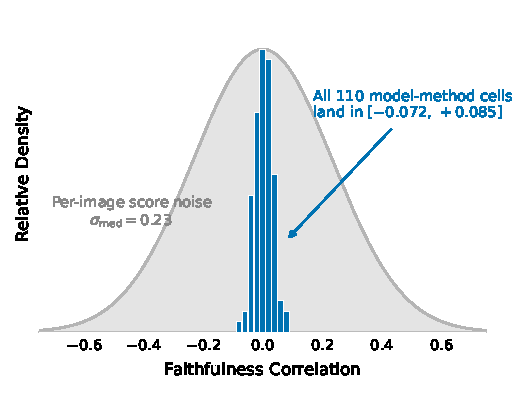
\includegraphics[width=\linewidth]{figures/hilrp/hilrp_fc_null.pdf}
  \caption{\textbf{FC cannot discriminate between attribution methods on modern ViTs.} Per-cell mean FC over all $118$ model-method cells (blue, peak-normalized) against the per-image score noise, a normal density at the median per-image $\sigma=0.23$ (gray). The entire between-method signal spans $[-0.072,+0.085]$ and sits deep inside the noise, so the metric scores good and bad localizers indistinguishably.}
  \label{fig:fc-noise}
\end{figure}

\begin{table}[!tbp]
  \centering
    \caption{\textbf{Benchmark results.} Pointing Game accuracy for 15
    attribution methods across 10 architectures, grouped into CNNs, isotropic
    ViTs, and hierarchical/hybrid ViTs. \nd\ = not applicable or not run.
    R50 $=$ ResNet-50, CNX $=$ ConvNeXt-B, ViT $=$ ViT-B, DeiT $=$ DeiT-B,
    MoV $=$ MobileViT-v2, EV1/EV2 $=$ EfficientViT-B1/B2, MxV $=$ MaxViT-S.}
  \label{tab:bigbench}
  \setlength{\tabcolsep}{1.6pt}
  \scriptsize
  \begin{tabular}{@{}l cc cc cccccc@{}}
    \toprule
    & \multicolumn{2}{c}{CNN} & \multicolumn{2}{c}{Isotropic ViT} & \multicolumn{6}{c}{Hierarchical / hybrid ViT} \\
    \cmidrule(lr){2-3}\cmidrule(lr){4-5}\cmidrule(lr){6-11}
    Method & R50 & CNX & ViT & DeiT & Swin & PVT & MoV & EV1 & EV2 & MxV \\
    \midrule
    Grad-CAM          & 0.98 & 1.00 & 0.93 & 0.90 & \textbf{1.00} & 0.84 & \textbf{1.00} & 0.70 & \underline{0.55} & \textbf{1.00} \\
    Grad-CAM++        & 0.97 & 0.95 & \underline{0.49} & 0.62 & \textbf{1.00} & 0.88 & \textbf{1.00} & \underline{0.44} & 0.56 & 0.80 \\
    Attn.\ Rollout   & \nd & \nd & 0.64 & \underline{0.48} & \nd & \nd & \nd & \nd & \nd & \nd \\
    Attention-grad    & \nd & \nd & 0.74 & 0.86 & \nd & \nd & \nd & \nd & \nd & \nd \\
    Saliency          & 0.82 & 0.73 & 0.65 & 0.54 & 0.62 & 0.62 & 0.90 & 0.86 & 0.66 & 0.58 \\
    Input$\times$Grad & 0.86 & 0.77 & 0.64 & 0.56 & 0.67 & 0.66 & 0.88 & 0.74 & 0.64 & 0.56 \\
    Integr.\ Grad    & 0.92 & 0.76 & 0.64 & 0.58 & 0.66 & 0.64 & 0.90 & 0.90 & 0.90 & 0.62 \\
    SmoothGrad        & 0.97 & 0.89 & 0.85 & 0.90 & 0.79 & 0.92 & 0.92 & 0.92 & 0.92 & 0.70 \\
    VarGrad           & 0.98 & 0.81 & 0.76 & 0.83 & 0.71 & 0.88 & 0.90 & 0.90 & 0.92 & 0.68 \\
    GradientSHAP      & 0.92 & 0.79 & 0.66 & 0.62 & 0.71 & 0.68 & 0.83 & 0.64 & 0.82 & 0.60 \\
    Occlusion         & 0.95 & 0.92 & 0.76 & 0.70 & 0.78 & 0.78 & 0.92 & \textbf{0.96} & 0.88 & 0.66 \\
    RISE              & 0.82 & 0.69 & 0.73 & 0.71 & 0.68 & 0.68 & 0.90 & 0.92 & 0.78 & 0.70 \\
    LIME              & 0.94 & 0.84 & 0.87 & 0.89 & 0.86 & 0.86 & 0.90 & 0.80 & 0.90 & 0.80 \\
    AttnLRP           & \nd & \nd & 0.78 & 0.84 & 0.98 & 0.80 & 0.95 & 0.84 & 0.93 & 0.89 \\
    \midrule
    \textbf{HiLRP (ours)} & \nd & \nd & 0.70 & 0.90 & 0.96 & \textbf{0.98} & 0.86 & \textbf{0.96} & \textbf{0.97} & 0.96 \\
    \bottomrule
  \end{tabular}
\end{table}

\subsection{Localization on Hierarchical and Hybrid ViTs}
\label{sec:localization}
We read the four hierarchical and hybrid columns of Table~\ref{tab:bigbench} together, since they span three mixing mechanisms: Swin-B (shifted window), PVT-v2-b2 (spatial reduction), EfficientViT-B2 (linear cross-covariance), and MobileViT-v2 (convolution hybrid).

HiLRP attains the highest cross-architecture mean Pointing score ($0.943$, against $0.861$ for the next best) and the smallest spread across backbones, and it is the only method that never falls to or below the random-point prior. It is not uniformly best: on MobileViT-v2 it is the lowest of the five methods compared ($0.860$), for the structural reason given in Sec.~\ref{sec:limitations}. However, Pointing Game accuracy alone is an insufficient discriminator. The metric is permissive on ImageNet-S (center-point prior $0.97$), so it saturates for CAM methods on architectures whose feature maps peak at the object center (Swin, MobileViT), while gradient methods vary by $0.30$ across architectures. HiLRP's advantage is sharpest where CAM's spatial assumption breaks. On EfficientViT, whose linear cross-covariance attention removes that assumption, Grad-CAM collapses to $0.551$, below the $0.61$ random-point prior, while HiLRP scores $0.970$; on PVT-v2 HiLRP reaches $0.980$ against Grad-CAM's $0.840$. On MobileViT and Swin, where Grad-CAM saturates the metric, HiLRP is competitive ($0.86$, $0.96$) and additionally provides stage-localized maps that CAM cannot (Sec.~\ref{sec:qualitative}), plus conservation guarantees on Swin (MobileViT is a designated extension, Sec.~\ref{sec:limitations}).

To confirm these gaps are not small-sample artifacts, we repeated both principal localization comparisons at $n{=}1000$ ImageNet-S images with paired per-image scoring, and on $1000$ images from the PASCAL VOC 2007~\cite{everingham2010voc} test set using its object bounding-box annotations. On ImageNet-S for EfficientViT, HiLRP reaches $0.936$ (95\% bootstrap confidence interval (CI) $[0.921,0.950]$) against Grad-CAM's $0.518$ ($[0.486,0.549]$); on PVT-v2, $0.958$ ($[0.945,0.970]$) against $0.846$ ($[0.823,0.868]$). In both legs the intervals do not overlap and the difference is significant under a paired McNemar test on the same images ($p<10^{-100}$ and $p<10^{-23}$). HiLRP localizes correctly on $437$ EfficientViT images where Grad-CAM fails, against $19$ the other way, and on $124$ against $12$ for PVT. The gap replicates on VOC: HiLRP scores $0.820$ ($[0.795,0.843]$) against Grad-CAM's $0.582$ ($[0.551,0.612]$, $p<10^{-40}$) on EfficientViT, and $0.865$ ($[0.844,0.886]$) against $0.621$ ($[0.591,0.650]$, $p<10^{-47}$) on PVT-v2. The failure of CAM on linear attention, and its recovery by HiLRP, therefore hold on a second dataset with a different annotation type. Because Pointing does not discriminate the top tier, we ground the central claim in two properties CAM lacks entirely: relevance conservation (Sec.~\ref{sec:conservation-validity}) and agreement with axiomatic Shapley values (Sec.~\ref{sec:shapley}).

\begin{figure}[!tbp]
  \centering
  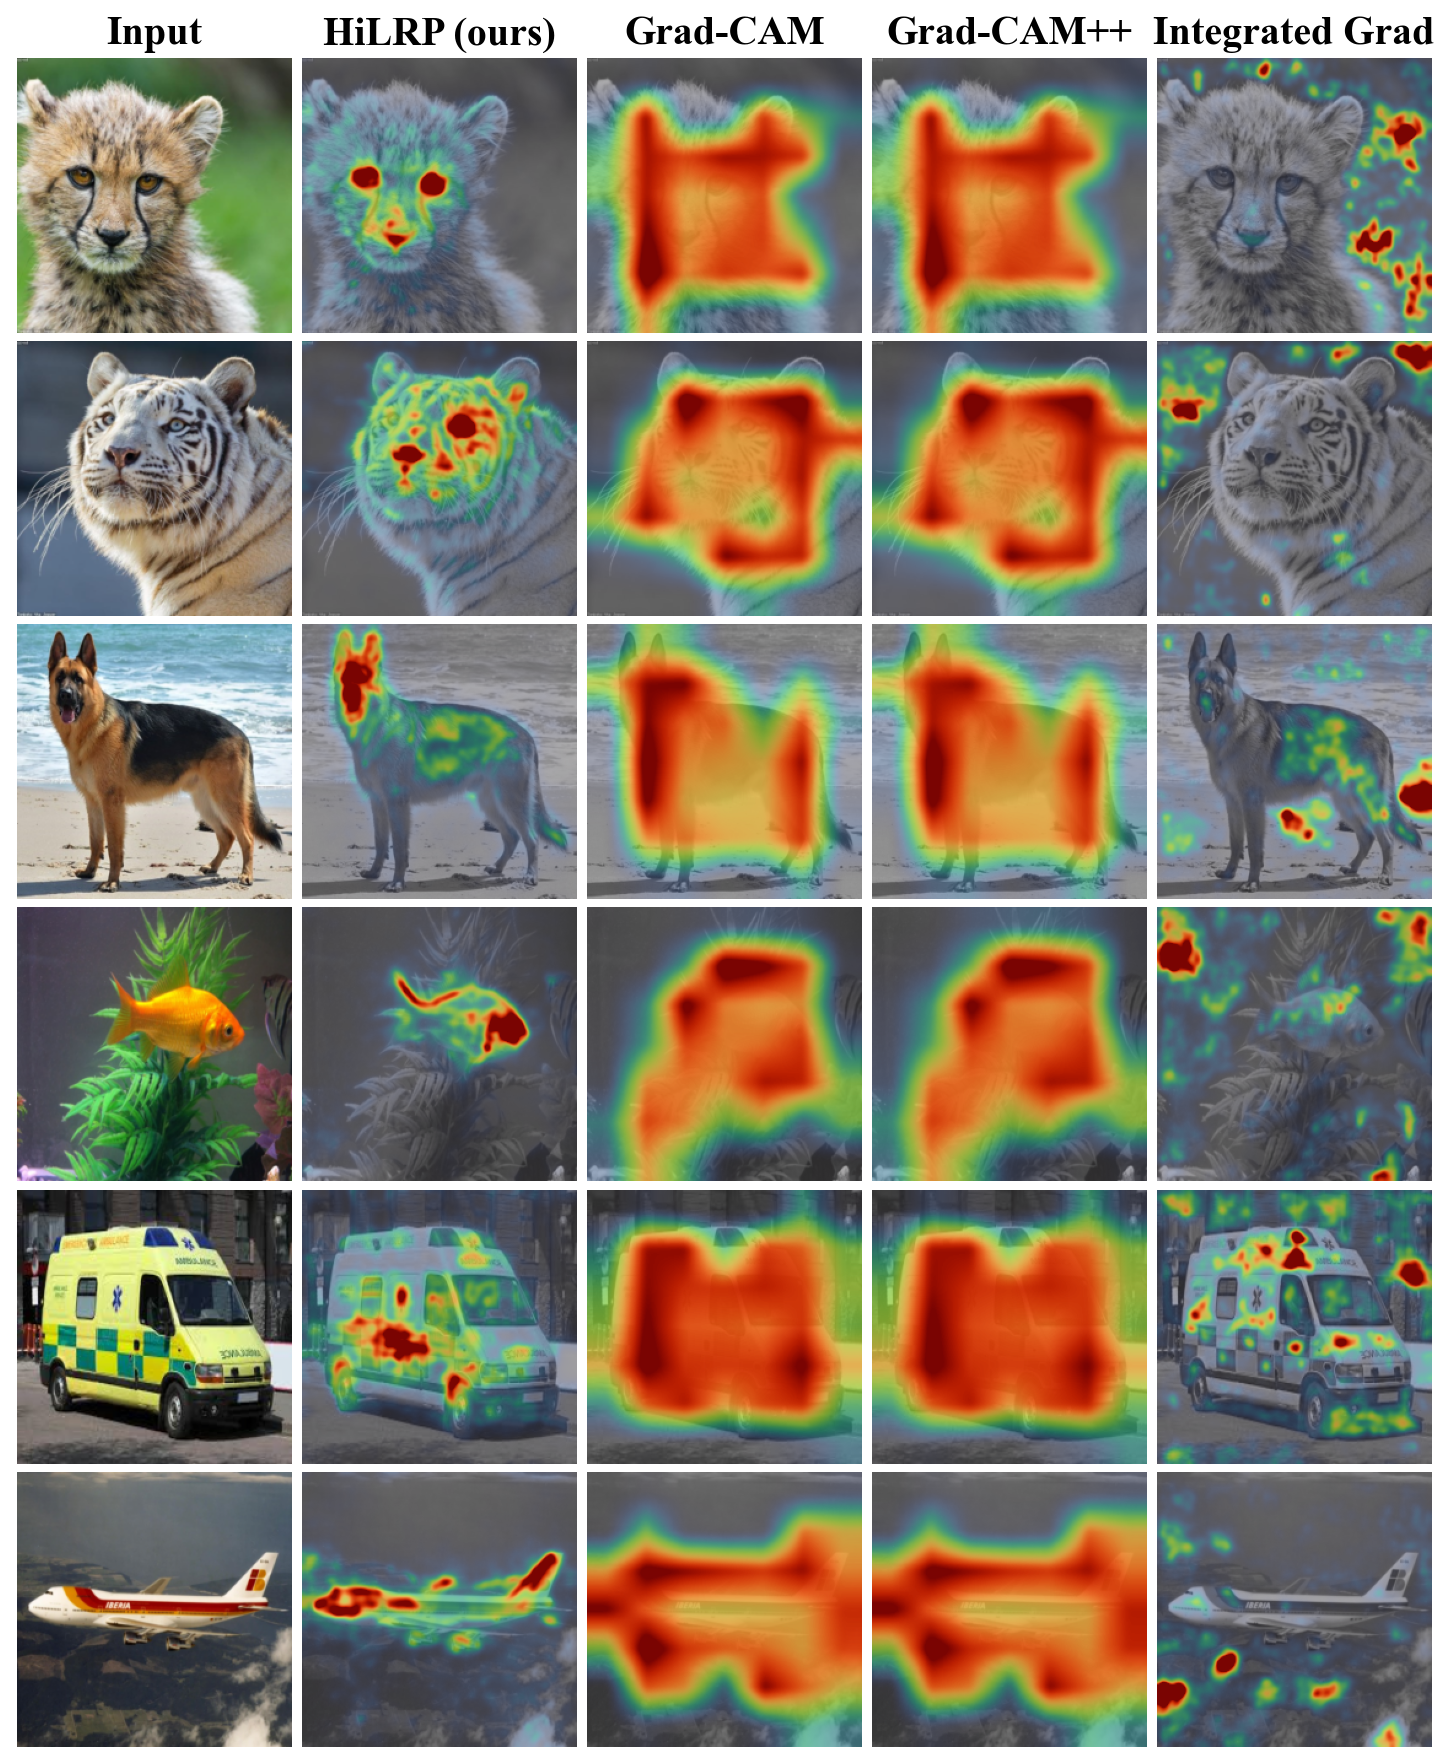
\includegraphics[width=\linewidth]{figures/bench/qualitative_gallery.png}
  \caption{\textbf{Qualitative comparison on PVT-v2-b2.} Heatmaps are shown over desaturated inputs for the predicted class. HiLRP provides more object-focused explanations, highlighting discriminative regions, while Grad-CAM, Grad-CAM++, and Integrated Gradients produce more diffuse or scattered attributions.}
  \label{fig:qualitative-comparison}
\end{figure}

\subsection{Why Grad-CAM Saturates the Pointing Game}
\label{sec:gradcam-blob}
Grad-CAM's perfect Pointing on Swin and MobileViT (Table~\ref{tab:bigbench}) is not evidence of precise localization; it is an artifact of the metric interacting with a low-resolution, center-biased map. Grad-CAM upsamples a $7{\times}7$ terminal feature map into a smooth blob whose peak, on a dataset of large centered objects, lands inside the object almost by construction. A content-free center-Gaussian blob that uses no model at all already scores a Pointing of $1.00$ on both Swin and MobileViT, equal to Grad-CAM. Grad-CAM's own maps correlate strongly with that Gaussian (Pearson $0.72$ on Swin, $0.63$ on MobileViT), and their center of mass sits within $11$--$21\%$ of the image center. HiLRP maps correlate only $0.14$--$0.25$ with it: they follow object structure rather than reproducing the dataset's spatial prior, as Fig.~\ref{fig:qualitative-comparison} shows. Grad-CAM therefore scores highly on the Pointing Game where the prior is strong and fails where it is not (EfficientViT, $0.551$), which is why Pointing is not treated as the deciding criterion.

\subsection{Mass-Based Localization and the Center-Prior Control}
\label{sec:energy-localization}
The Pointing Game reads only the $\arg\max$ of a map. A metric that uses the whole map is potentially more informative, so we add three such measures: \emph{energy}, the fraction of positive relevance falling inside the ground-truth region; the threshold-free average precision of $|R|$ treated as a per-pixel detector of that region; and the best IoU over a sweep of thresholds. All three are computed on the same $1000$ ImageNet-S images, paired per image, against the object boxes. We score a \emph{content-free center Gaussian} alongside them as a control, since it uses no model, no gradient, and no image. On this box-annotated set the mean object area is $0.591$, so a uniform map scores exactly that energy; we therefore report the \emph{excess} over the area, which is zero for a uniform map. Table~\ref{tab:energy} gives the result, which admits two separate observations.

\textbf{AP and IoU are confounded by the same prior that saturates Pointing.} The model-free center Gaussian scores AP $0.845$ and IoU $0.555$, higher than HiLRP on all four backbones and higher than Grad-CAM on PVT ($0.826$) and EfficientViT ($0.630$). A metric that ranks a blob computed without looking at the image above nearly every model-derived attribution is not measuring attribution quality here; it is measuring how closely a map's support matches the extent of a large centered object. This extends the diagnosis of Sec.~\ref{sec:gradcam-blob} from Pointing to the two most common mask-based alternatives, so neither is adopted as a primary criterion.

\textbf{Energy excess, referenced to that control, does discriminate.} HiLRP exceeds the center-Gaussian on every architecture, from $+0.159$ on Swin to $+0.211$ on PVT (paired Wilcoxon $p<2.4{\times}10^{-3}$ throughout), whereas Grad-CAM falls \emph{below} the model-free control on PVT ($+0.124$ versus $+0.137$, $p=2.4{\times}10^{-16}$) and far below it on EfficientViT ($-0.049$, $p=1.2{\times}10^{-80}$), where it places less relevance mass inside the object than a uniform map would. Across the four backbones HiLRP's excess spans $0.052$ and Grad-CAM's spans $0.266$, a five-fold difference in cross-architecture spread. This is the consistency claim of Sec.~\ref{sec:localization} measured against a proper null rather than asserted.

Two cases do not favor HiLRP. Grad-CAM's energy excess is higher than HiLRP's on Swin ($+0.179$ versus $+0.159$, $p=5.5{\times}10^{-47}$), and on MobileViT the two are statistically indistinguishable ($+0.217$ versus $+0.203$, $p=0.33$). The pattern is the architecture-dependence this paper reports throughout: where CAM's terminal feature map is meaningful it remains a strong localizer, and where that assumption fails it drops beneath a control that uses no model at all. Only HiLRP stays above the control everywhere, which is the property a general-purpose attributor needs.

\begin{table}[!tbp]
  \centering
  \caption{\textbf{Mass-based localization against a model-free control}
  ($n{=}1000$ ImageNet-S, paired). \emph{Energy excess} is the fraction of
  positive relevance inside the object minus the object's area ($0.591$), so a
  uniform map scores $0$. The \textsc{center} row is a center Gaussian computed
  without the model or the image. Underlined entries fall below that control;
  best energy excess per backbone in bold.}
  \label{tab:energy}
  \setlength{\tabcolsep}{4pt}
  \footnotesize
  \begin{tabular}{@{}l l c c c@{}}
    \toprule
    Backbone & Method & Energy excess \up & AP & IoU \\
    \midrule
    \multicolumn{5}{@{}l}{\emph{Model-free reference}} \\
    \quad \textsc{center} Gaussian & \nd & $+0.137$ & $0.845$ & $0.555$ \\
    \midrule
    \multirow{2}{*}{Swin-B}
      & HiLRP    & $+0.159$ & $0.745$ & $0.438$ \\
      & Grad-CAM & $\best{+0.179}$ & $0.884$ & $0.587$ \\
    \addlinespace
    \multirow{2}{*}{PVT-v2-b2}
      & HiLRP    & $\best{+0.211}$ & $0.796$ & $0.486$ \\
      & Grad-CAM & \underline{$+0.124$} & $0.826$ & $0.564$ \\
    \addlinespace
    \multirow{2}{*}{EfficientViT-B2}
      & HiLRP    & $\best{+0.200}$ & $0.757$ & $0.456$ \\
      & Grad-CAM & \underline{$-0.049$} & $0.630$ & $0.489$ \\
    \addlinespace
    \multirow{2}{*}{MobileViT-v2}
      & HiLRP    & $+0.203$ & $0.777$ & $0.486$ \\
      & Grad-CAM & $\best{+0.217}$ & $0.877$ & $0.589$ \\
    \midrule
    \multicolumn{2}{@{}l}{Cross-architecture spread}
      & \multicolumn{3}{l}{HiLRP $0.052$ \quad Grad-CAM $0.266$} \\
    \bottomrule
  \end{tabular}
\end{table}

\subsection{Conservation Validity vs.\ the Naive Lineage}
\label{sec:conservation-validity}
The central claim of HiLRP is not a Pointing win but \emph{conservation validity}: on hierarchical and hybrid architectures, none of the attribution methods evaluated here produces relevance that conserves to the prediction. AttnLRP~\cite{achtibat2024attnlrp} defines rules only for isotropic transformers. Explaining a hierarchical model with that method therefore requires retaining its flat-transformer rules unchanged and leaving the hierarchical operations to the unmodified gradient computation, which is the configuration we evaluate below. We evaluate this ``naive'' extension against HiLRP under an identical backend, granting the naive baseline the same batch-norm canonization and preprocessing, and withholding only HiLRP's contributions: the resolution-reduction rules, the normalization-subclass handling, and the non-\textsc{gelu} activation rules.

Table~\ref{tab:conservation} reports, for the five attention-based hierarchical backbones, the relevance sum at the input-adjacent capture (normalized by the logit; $1.0$ is exact) alongside the Pointing score, for the naive AttnLRP extension and for HiLRP. The naive extension produces \emph{degenerate} relevance on every architecture: it inflates the sum by $3.1\times$ on Swin and drives it to \emph{exactly zero} at depth on the other four, because their scale-invariant normalizations, left unpatched, force the per-token relevance sum to vanish; on MaxViT the failure reaches the head. The naive maps nonetheless still \emph{point} well ($0.80$--$0.98$, sometimes above HiLRP), because a zero-sum map still has an $\arg\max$. Pointing therefore cannot detect that these maps are not conservation-based attributions at all: their region contributions do not sum to the logit, violating the completeness property that is LRP's sole justification.

HiLRP keeps a bounded, non-degenerate sum on all five: $0.77$ on Swin, $0.38$ on PVT, and $0.16$ on MaxViT under the global $\gamma{=}0.25$, and $0.13$ and $0.35$ on EfficientViT-B1 and B2 once their deep convolutional stack is given a lower stabilizer ($\gamma_{\text{conv}}{=}0.05$; the global $0.25$ over-concentrates on positive contributions and zeroes the input relevance, while $\gamma_{\text{conv}}$ below ${\sim}0.03$ swings into $\varepsilon$-cancellation instability). The sums below $1.0$ are the controlled $\gamma$-rule deviation, the pixel-level cost quantified in Sec.~\ref{sec:limitations}. The convolution-hybrid MobileViT-v2 falls outside this attention-based set, combining depthwise convolutions, a global \textsc{GroupNorm}, and channel gating, so it needs primitives beyond those used here; we treat it as an extension rather than force a claim (Sec.~\ref{sec:limitations}). Classic LRP~\cite{bach2015lrp} does not run on any of these \texttt{timm} backbones (unsupported layer types).

\begin{table}[!tbp]
  \centering
  \caption{\textbf{Conservation validity.} Pointing / input-level relevance sum (normalized by the logit; $1.0$ exact), $n{=}100$. The naive extension is degenerate everywhere (zeroed or inflated $3.08\times$); HiLRP keeps a bounded, non-degenerate sum on all five attention-based backbones. The convolution-hybrid MobileViT-v2 is treated separately as an extension (Sec.~\ref{sec:limitations}).}
  \label{tab:conservation}
  \setlength{\tabcolsep}{4pt}
  \begin{tabular}{l cc}
    \toprule
    Backbone & Naive AttnLRP (pt / cons) & \textbf{HiLRP} (pt / cons) \\
    \midrule
    Swin-B          & 0.98 / $3.08$ (inflated) & 0.96 / $0.77$ \\
    PVT-v2-b2       & 0.80 / $0.00$ (zeroed)   & \textbf{0.98} / $0.38$ \\
    EfficientViT-B1 & 0.84 / $0.00$ (zeroed)   & \textbf{0.96} / $0.13$ \\
    EfficientViT-B2 & 0.93 / $0.00$ (zeroed)   & \textbf{0.97} / $0.35$ \\
    MaxViT-S        & 0.89 / $0.00$ (broken)   & \textbf{0.96} / $0.16$ \\
    \bottomrule
  \end{tabular}
\end{table}

We also validate the rules directly in a float64 reference implementation: the patch-merging rule conserves to $3\times10^{-16}$, the shifted-window mask leaks ${\sim}10^{-43}$ of relevance (structurally zero), and the conditional equivariance theorem holds to $<10^{-8}$ under the true symmetry group. On the pretrained Swin-B, Fig.~\ref{fig:conservation-stages} traces the relevance sum through every resolution stage. It stays near unity across the token grid and the merged stages and returns to $1.00$ at the head; only the $z^+$/$\gamma$ rule on the convolutional patch stem introduces the measured pixel-level deviation.

\begin{figure}[!tbp]
  \centering
  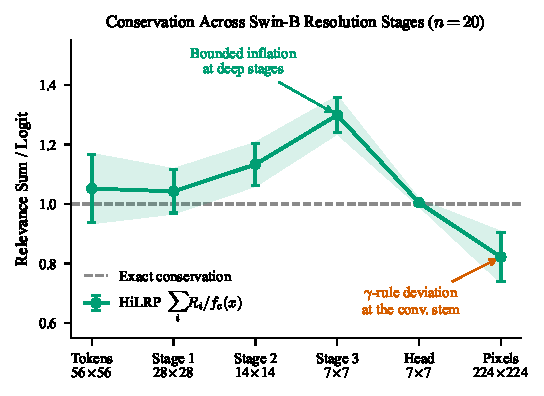
\includegraphics[width=\linewidth]{figures/hilrp/conservation_stages}
  \caption{\textbf{HiLRP relevance is conserved through the hierarchy.}
  Relevance sum over the target logit, $\sum_i R_i/f_c(x)$, at each Swin-B
  resolution stage ($n{=}20$), where $1.0$ denotes exact conservation.}
  \label{fig:conservation-stages}
\end{figure}

\subsection{Segment-Shapley Agreement}
\label{sec:shapley}
Because Pointing does not discriminate the top tier and FC is uninformative on robust ViTs (Sec.~\ref{sec:baseline-landscape}), we adopt agreement with sampled permutation Shapley values as the primary evidence. Shapley values are the unique attribution satisfying efficiency, symmetry, the null-player property, and additivity. We estimate them over SLIC superpixel segments with blur infill (avoiding out-of-distribution black patches) at $m{=}64$ permutations per image, and correlate each method's per-segment attribution against the reference (Spearman $\rho$). Exact SHAP and KernelSHAP are infeasible here, since the coalition space over image regions is exponential, so the sampled-permutation estimator serves as the axiomatic reference rather than as a competing attribution method; GradientSHAP, which does scale to these depths, is included as a benchmark baseline instead.

Table~\ref{tab:shapley} reports the agreement, and the $n{=}50$ intervals make its structure precise. On Swin and PVT, where Grad-CAM works, HiLRP and Grad-CAM are statistically indistinguishable (on Swin, HiLRP $0.528$, 95\% bootstrap CI $[0.47,0.58]$, against Grad-CAM $0.515$ $[0.47,0.56]$, paired Wilcoxon $p=0.45$), and both exceed the gradient methods, whose intervals lie below $0.35$. The separation appears on EfficientViT, whose linear attention removes the spatial heuristic: Grad-CAM's Shapley agreement collapses to $0.077$ while HiLRP holds $0.417$, mirroring the localization result. The claim is therefore not that HiLRP outscores Grad-CAM on every backbone, but that it is the only method whose agreement stays high across all three. Localization and Shapley agreement, two measures computed independently of each other, tell one story.

\begin{table}[!tbp]
  \centering
  \caption{\textbf{Shapley Agreement.} Spearman agreement with sampled Shapley values over image segments ($n{=}50$ images, $m{=}64$ permutations). Higher is better. Per-cell 95\% bootstrap intervals are approximately $\pm0.06$, so only the large EfficientViT gap between HiLRP ($0.417$) and Grad-CAM ($0.077$) is statistically separated; the Swin and PVT HiLRP-vs-Grad-CAM differences lie within noise, while both exceed the gradient baselines.}
  \label{tab:shapley}
  \setlength{\tabcolsep}{5pt}
  \begin{tabular}{l c c c}
    \toprule
    Method & Swin-T & PVT-v2 & EfficientViT-B2 \\
    \midrule
    \textbf{HiLRP (Ours)} & \textbf{0.528} & \textbf{0.531} & \textbf{0.417} \\
    Grad-CAM & 0.515 & 0.449 & 0.077 \\
    Integrated Grads & 0.192 & 0.279 & 0.281 \\
    SmoothGrad & 0.312 & 0.260 & 0.321 \\
    Saliency & 0.214 & 0.137 & 0.240 \\
    \bottomrule
  \end{tabular}
\end{table}

\subsection{The Perturbation Metrics, and Where They Disagree}
\label{sec:perturbation-metrics}
As shown in Sec.~\ref{sec:baseline-landscape}, FC does not
separate attribution methods on these architectures, and conservation validity
and Shapley agreement are therefore adopted as the primary evaluation axes. That argument would be incomplete were the paper to omit
the perturbation metrics the attribution literature usually reports, so we
report all four of them, together with the control that reveals what they
measure. Average Drop (AD) and Average Increase (AI) keep the top $20\%$ of
attributed pixels and read the change in the target probability; Deletion (Del)
and Insertion (Ins) remove or add pixels most-important-first and integrate the
resulting curve. The
control is a random map generated at a coarse ($14{\times}14$, upsampled) and a
fine ($224{\times}224$) resolution, using neither the model nor the image.

Table~\ref{tab:adai} reports the result, which separates into two findings.

\textbf{The metrics are not uninformative, and the previously reported failure
mode does not reproduce here.} On all three backbones both real methods
outperform both random controls on Average Drop, and the random maps never
outperform them on Deletion. Yuan et~al.~\cite{yuan2025fourchar} observe that on convolutional backbones a
sufficiently fine random map outscores every attribution method under Deletion.
That behavior is not observed on the ViT backbones evaluated here. Their result
and ours are consistent in their implication, namely that the perturbation
family requires a model-free control before its scores can be interpreted, but
they are separate observations obtained on different architecture families.

\textbf{However, these metrics contradict alternative evaluations on the
architectures where the failure modes are most pronounced.} On Swin and PVT-v2
they agree with the rest of the paper:
HiLRP has the best Average Drop, Average Increase, and Deletion on both, and
Insertion on Swin. On EfficientViT-B2 they invert. Grad-CAM scores better
Average Drop ($61.5$ against $88.5$), Average Increase, and Insertion, even
though on that same backbone and the same images Grad-CAM localizes below the
random-point prior (Sec.~\ref{sec:localization}), agrees with sampled Shapley at
only $0.077$ (Sec.~\ref{sec:shapley}), places \emph{more} relevance inside the
object for the model's least likely class than for its predicted class, and
returns positively correlated maps for opposite classes
(Sec.~\ref{sec:class-sensitivity}). Three axes computed independently of each
other say Grad-CAM has failed on linear attention; the perturbation metrics rank
it first.

The exact mechanism driving this discrepancy remains a subject for future investigation. Two candidates are apparent in our own measurements: keeping the top $20\%$ of a heavy-tailed pixel map, which
is the form HiLRP produces on this backbone (Sec.~\ref{sec:class-sensitivity}),
retains a scattered pixel set, whereas thresholding a smooth CAM blob retains a
connected region, and a connected region is the more in-distribution input;
and zeroing pixels is itself an out-of-distribution operation whose severity
differs by architecture. The claim made here is narrower: on EfficientViT-B2, the backbone for which the
independent evidence of a method's failure is strongest, the perturbation
metrics rank that method first, so they cannot serve as the deciding criterion
for this comparison. This is the argument of Sec.~\ref{sec:baseline-landscape}
supported by the corresponding measurements.

\begin{table}[!tbp]
  \centering
  \caption{\textbf{Perturbation metrics with a model-free control}
  ($n{=}100$, paired). AD and AI are percentages. \textsc{random} rows use
  neither the model nor the image. Best real method per backbone and column in
  bold; underlined entries mark the EfficientViT case discussed in the text.}
  \label{tab:adai}
  \setlength{\tabcolsep}{4pt}
  \footnotesize
  \begin{tabular}{@{}l l r r r r@{}}
    \toprule
    Backbone & Method & AD \down & AI \up & Del \down & Ins \up \\
    \midrule
    \multirow{4}{*}{Swin-B}
      & \textbf{HiLRP}  & \best{32.2} & \best{14.0} & \best{0.286} & \best{0.580} \\
      & Grad-CAM        & 41.4 & 5.0 & 0.335 & 0.566 \\
      & \textsc{random} coarse & 55.8 & 5.0 & 0.492 & 0.500 \\
      & \textsc{random} fine   & 81.4 & 0.0 & 0.394 & 0.399 \\
    \addlinespace
    \multirow{4}{*}{PVT-v2-b2}
      & \textbf{HiLRP}  & \best{36.4} & \best{13.0} & \best{0.199} & 0.566 \\
      & Grad-CAM        & 37.4 & 11.0 & 0.318 & \best{0.586} \\
      & \textsc{random} coarse & 71.5 & 1.0 & 0.408 & 0.413 \\
      & \textsc{random} fine   & 92.2 & 0.0 & 0.327 & 0.326 \\
    \addlinespace
    \multirow{4}{*}{EfficientViT-B2}
      & \textbf{HiLRP}  & 88.5 & 3.0 & \best{0.275} & 0.330 \\
      & Grad-CAM        & \underline{61.5} & \underline{13.0} & 0.568 & \underline{0.637} \\
      & \textsc{random} coarse & 93.6 & 0.0 & 0.451 & 0.464 \\
      & \textsc{random} fine   & 96.3 & 1.0 & 0.398 & 0.392 \\
    \bottomrule
  \end{tabular}
\end{table}

\subsection{Class Sensitivity and Misclassified Samples}
\label{sec:class-sensitivity}
Localization scores cannot distinguish an explanation of a \emph{class} from a
detector of the \emph{salient object}: a map that finds the object scores well
whatever class it was asked about. We probe this directly. On the same image we
attribute the predicted class and then the model's \emph{least likely} class,
the one with the lowest logit. The usual top-1 against top-2 probe is
the wrong test on single-object data, since both classes are supported by the
same object and high agreement is expected; the bottom-1 class is defined by the
model itself and needs no semantic-distance heuristic.

A signed, conservation-valid attribution makes a falsifiable prediction here. If
the relevance decomposes the logit, then evidence that raises the predicted
class must \emph{lower} the class the model ranks last, so the sign of the
relevance inside the object should invert. Table~\ref{tab:class-sensitivity}
reports the result over $100$ ImageNet-S images with segmentation masks. It does
invert, on every image of all three backbones: mean in-object relevance is
positive for the predicted class and negative for the least likely class in
$100/100$ cases per backbone, and the two maps are near mirror images on Swin
($\rho=-0.988$) and PVT ($\rho=-0.980$). Fig.~\ref{fig:class-sensitivity} shows
the effect: the same object structure is traced in both maps, with the sign
reversed.

Grad-CAM cannot represent this inversion. Its map is $\mathrm{ReLU}$-rectified by
construction, so it has no negative range, and the sign test is therefore
structurally inapplicable to it rather than failed by it. The fair comparison is the map
correlation, and there the architecture-dependence of Sec.~\ref{sec:localization}
reappears on a third, independent axis. On Swin and PVT, Grad-CAM's two class
maps are weakly anti-correlated ($-0.34$, $-0.38$), so it retains some class
specificity. On EfficientViT-B2 the correlation turns \emph{positive}
($+0.137$): the map for the model's least likely class agrees with the map for
its predicted class, and places \emph{more} mass inside the object ($+1.27$
against $+1.09$). Grad-CAM is not class-sensitive at all on this backbone. Its
localization failure, its reduced Shapley agreement, and its absent class
sensitivity constitute the same underlying failure measured along three axes.

The evidence is weaker on one of the three backbones, and the margin is reported
rather than report only the direction. On EfficientViT-B2 HiLRP has the correct
sign on every image, but the magnitudes are small ($+0.093$ against $-0.051$)
and the map correlation is only $-0.182$, against $-0.98$ on the other two
backbones.
The reduced convolutional stabilizer that backbone requires
($\gamma_{\text{conv}}{=}0.05$, Sec.~\ref{sec:implementation}) yields a noisier
pixel map, and the class-sensitivity signal degrades with it. The direction is
right on every image; the margin is not comparable to Swin and PVT.

\textbf{Misclassified samples.} When a model is wrong, an explanation should
follow the model rather than the label. On the misclassified subset we attribute
both the predicted and the ground-truth class. The two maps agree strongly
(Spearman $+0.974$ on Swin with $n{=}10$, $+0.950$ on PVT with $n{=}12$,
$+0.686$ on EfficientViT with $n{=}9$), and both place positive evidence on the
object. This is a negative result for the probe, and the cause is the data
rather than the method: ImageNet-S images contain a single dominant object, so a
misclassification is almost always a confusion between two classes that the same
object supports, and no attribution could separate them from this evidence. The
probe would discriminate on multi-object scenes, where the predicted and
ground-truth classes correspond to different image regions. We report it as a
limitation of the evaluation set (Sec.~\ref{sec:limitations}) rather than
present the agreement as a positive finding.

\begin{table}[!tbp]
  \centering
  \caption{\textbf{Class sensitivity} ($n{=}100$ ImageNet-S images with masks).
  Each image is attributed for the predicted class and for the model's least
  likely class. \emph{Map corr.}\ is the Pearson correlation between the two
  maps; \emph{In-mask} is mean relevance inside the object mask, normalized by
  the map's mean absolute value; \emph{Flip} counts images whose in-mask
  evidence changes sign between the two classes$^{\dagger}$.}
  \label{tab:class-sensitivity}
  \setlength{\tabcolsep}{4pt}
  \footnotesize
  \begin{tabular}{@{}l l r r r c@{}}
    \toprule
    & & & \multicolumn{2}{c}{In-mask relevance} & \\
    \cmidrule(lr){4-5}
    Backbone & Method & Map corr. & Pred. & Least-likely & Flip \\
    \midrule
    \multirow{2}{*}{Swin-B}
      & \textbf{HiLRP} & $\best{-0.988}$ & $+1.37$ & $-1.30$ & $100/100$ \\
      & Grad-CAM       & $-0.341$        & $+1.77$ & $+0.53$ & \nd$^{\dagger}$ \\
    \addlinespace
    \multirow{2}{*}{PVT-v2-b2}
      & \textbf{HiLRP} & $\best{-0.980}$ & $+1.74$ & $-1.70$ & $100/100$ \\
      & Grad-CAM       & $-0.381$        & $+1.41$ & $+0.39$ & \nd$^{\dagger}$ \\
    \addlinespace
    \multirow{2}{*}{EfficientViT-B2}
      & \textbf{HiLRP} & $\best{-0.182}$ & $+0.09$ & $-0.05$ & $100/100$ \\
      & Grad-CAM       & \underline{$+0.137$} & $+1.09$ & $+1.27$ & \nd$^{\dagger}$ \\
    \bottomrule
  \end{tabular}
  \\[2pt]
  \footnotesize{$^{\dagger}$Grad-CAM's output is $\mathrm{ReLU}(\sum_k w_k A_k)$,
  which is non-negative everywhere, so it cannot represent evidence \emph{against}
  a class. This is a property of the method, not a measurement outcome. The
  underlined EfficientViT entry is the failure discussed in the text: the two
  class maps are positively correlated there, so the explanation does not depend
  on the class being explained.}
\end{table}

\begin{figure}[!tbp]
  \centering
  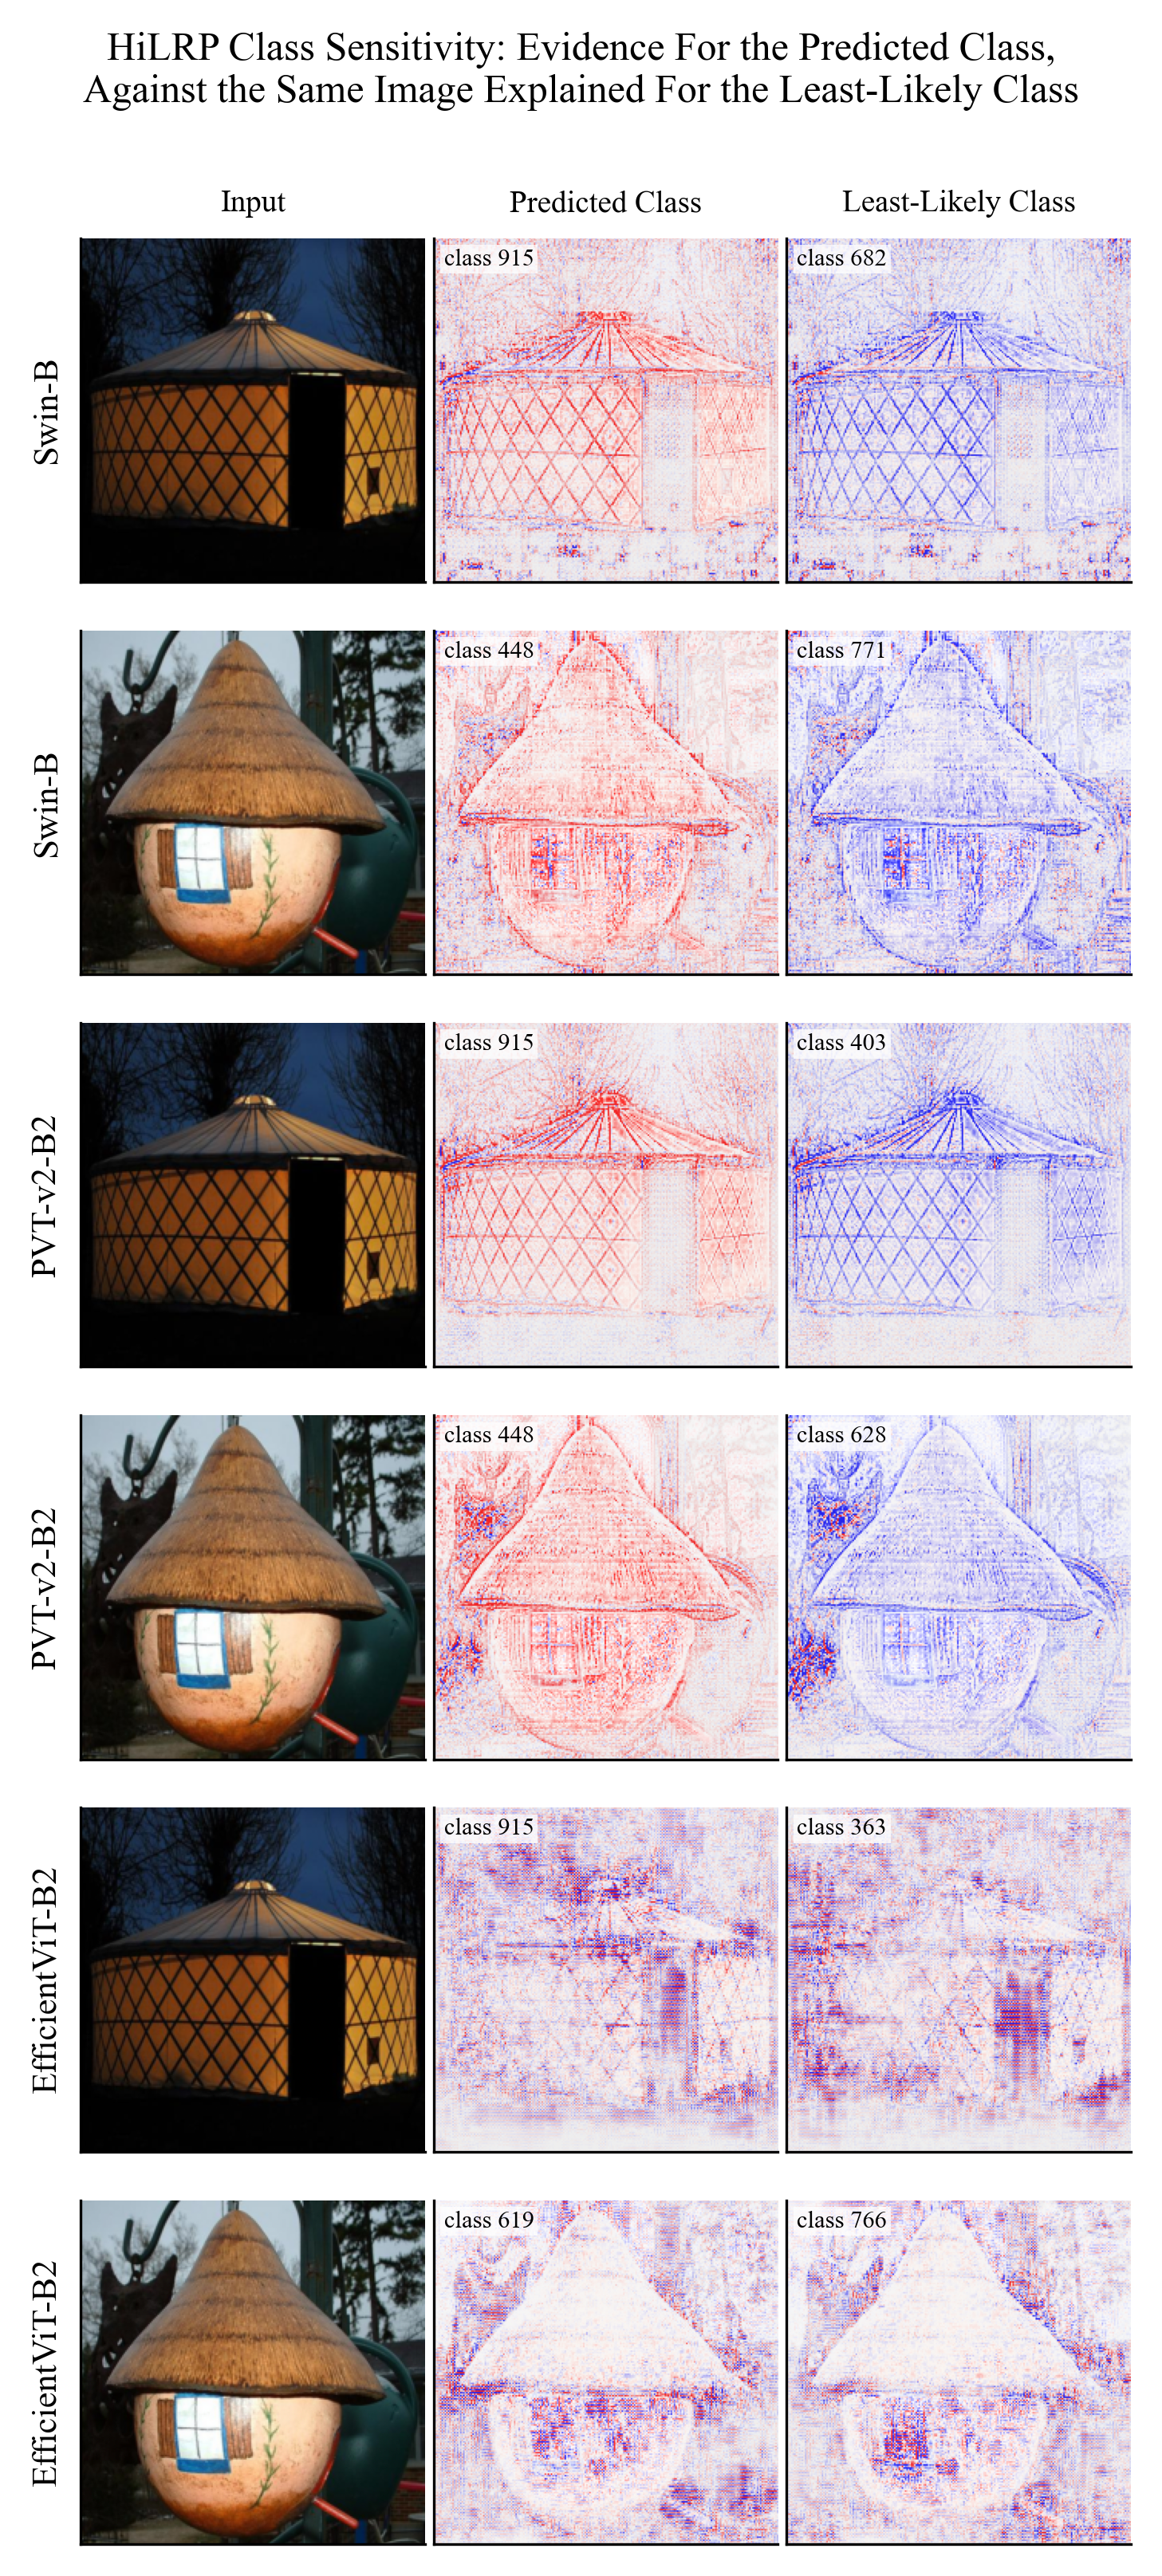
\includegraphics[width=\linewidth]{figures/hilrp/class_sensitivity.png}
  \caption{\textbf{The sign of the evidence follows the class.} Each row shows
  one image and one backbone: input, HiLRP relevance for the predicted class,
  and relevance for the model's least likely class. Red is positive relevance,
  blue negative. Panels are scaled independently so that the sign remains
  legible; magnitudes are given in Table~\ref{tab:class-sensitivity}.}
  \label{fig:class-sensitivity}
\end{figure}

\subsection{Sanity Check: Parameter Randomization}
\label{sec:sanity}
An attribution method whose output is invariant to randomization of the model's
learned parameters cannot be reflecting the behavior of that model, and is
instead responding to properties of the input alone. Edge detectors illustrate
the concern directly: they satisfy every localization criterion while depending
on no learned parameter at all~\cite{adebayo2018sanity}. We apply both protocols
of this check. In the \emph{independent} protocol one block is randomized and
then restored; in the \emph{cascading} protocol blocks are randomized
cumulatively from the output backwards. In each case we recompute the
attribution for the class the intact model predicted and compare it with the
intact map. Weights are redrawn from a Gaussian matched to each parameter's own
standard deviation, so the scale is preserved and only the learned structure is
destroyed. We confirmed the randomization takes effect rather than silently
failing: the predicted class changes at every block, with maximum logit
deviations of $7.9$ to $11.9$.

Table~\ref{tab:sanity} reports the cascading protocol over $50$ images, and
Fig.~\ref{fig:sanity} shows both. HiLRP passes: agreement with the intact map
falls monotonically as more of the network is destroyed, from $0.99$ to $0.20$
on Swin and $0.92$ to $0.22$ on PVT, and the maps degrade visibly into noise
once the middle stages are reached.

Notably, the first row indicates that randomizing only the classifier head
leaves the magnitude map almost unchanged ($\rho_{|R|}=0.99$ on Swin), which
considered in isolation would suggest that the attribution is independent of the
classifier. The signed map indicates the opposite: agreement falls immediately
from $1.0$ to $-0.12$ on Swin and $-0.05$ on PVT. Both measurements are correct
and they quantify different properties. The intact backbone continues to select
the same pixels, so the magnitude structure is preserved; the class those pixels
support, however, is determined by the head, so randomizing the head inverts and
scrambles the sign. This is the same property that
Sec.~\ref{sec:class-sensitivity} measures in the complementary direction, where
the sign inverts when the explained class changes.

It follows that the standard sanity check, which by convention compares
magnitude maps, systematically understates the model-sensitivity of a signed
attribution, and would score a method that discards sign as \emph{more}
sensitive than one that keeps it. We therefore report both columns. We are not
aware of this distinction being drawn in previous applications of the check, and
suggest that signed attributions be evaluated on the signed map.

\begin{table}[!tbp]
  \centering
  \caption{\textbf{Parameter-randomization sanity check}, cascading protocol,
  $n{=}50$ ImageNet-S images. Each row randomizes the named block \emph{in
  addition} to every block above it, moving from the output towards the input.
  $\rho_{|R|}$ and $\rho_{R}$ are the Spearman correlations of the magnitude and
  signed maps against the intact attribution. Lower is better in both.}
  \label{tab:sanity}
  \setlength{\tabcolsep}{5pt}
  \footnotesize
  \begin{tabular}{@{}l c c c c@{}}
    \toprule
    & \multicolumn{2}{c}{Swin-B} & \multicolumn{2}{c}{PVT-v2-b2} \\
    \cmidrule(lr){2-3}\cmidrule(lr){4-5}
    Randomized through & $\rho_{|R|}$ \down & $\rho_{R}$ \down & $\rho_{|R|}$ \down & $\rho_{R}$ \down \\
    \midrule
    (intact)      & $1.000$ & $1.000$ & $1.000$ & $1.000$ \\
    head          & $0.986$ & $-0.122$ & $0.922$ & $-0.053$ \\
    \quad + stage 3     & $0.811$ & $+0.078$ & $0.737$ & $-0.229$ \\
    \quad + stage 2     & $0.333$ & $+0.014$ & $0.375$ & $-0.014$ \\
    \quad + stage 1     & $0.241$ & $+0.002$ & $0.252$ & $-0.005$ \\
    \quad + stage 0     & $0.224$ & $+0.003$ & $0.219$ & $-0.002$ \\
    \quad + patch embed & $\best{0.198}$ & $\best{+0.000}$ & $\best{0.219}$ & $\best{-0.002}$ \\
    \bottomrule
  \end{tabular}
\end{table}

\begin{figure*}[!tbp]
  \centering
  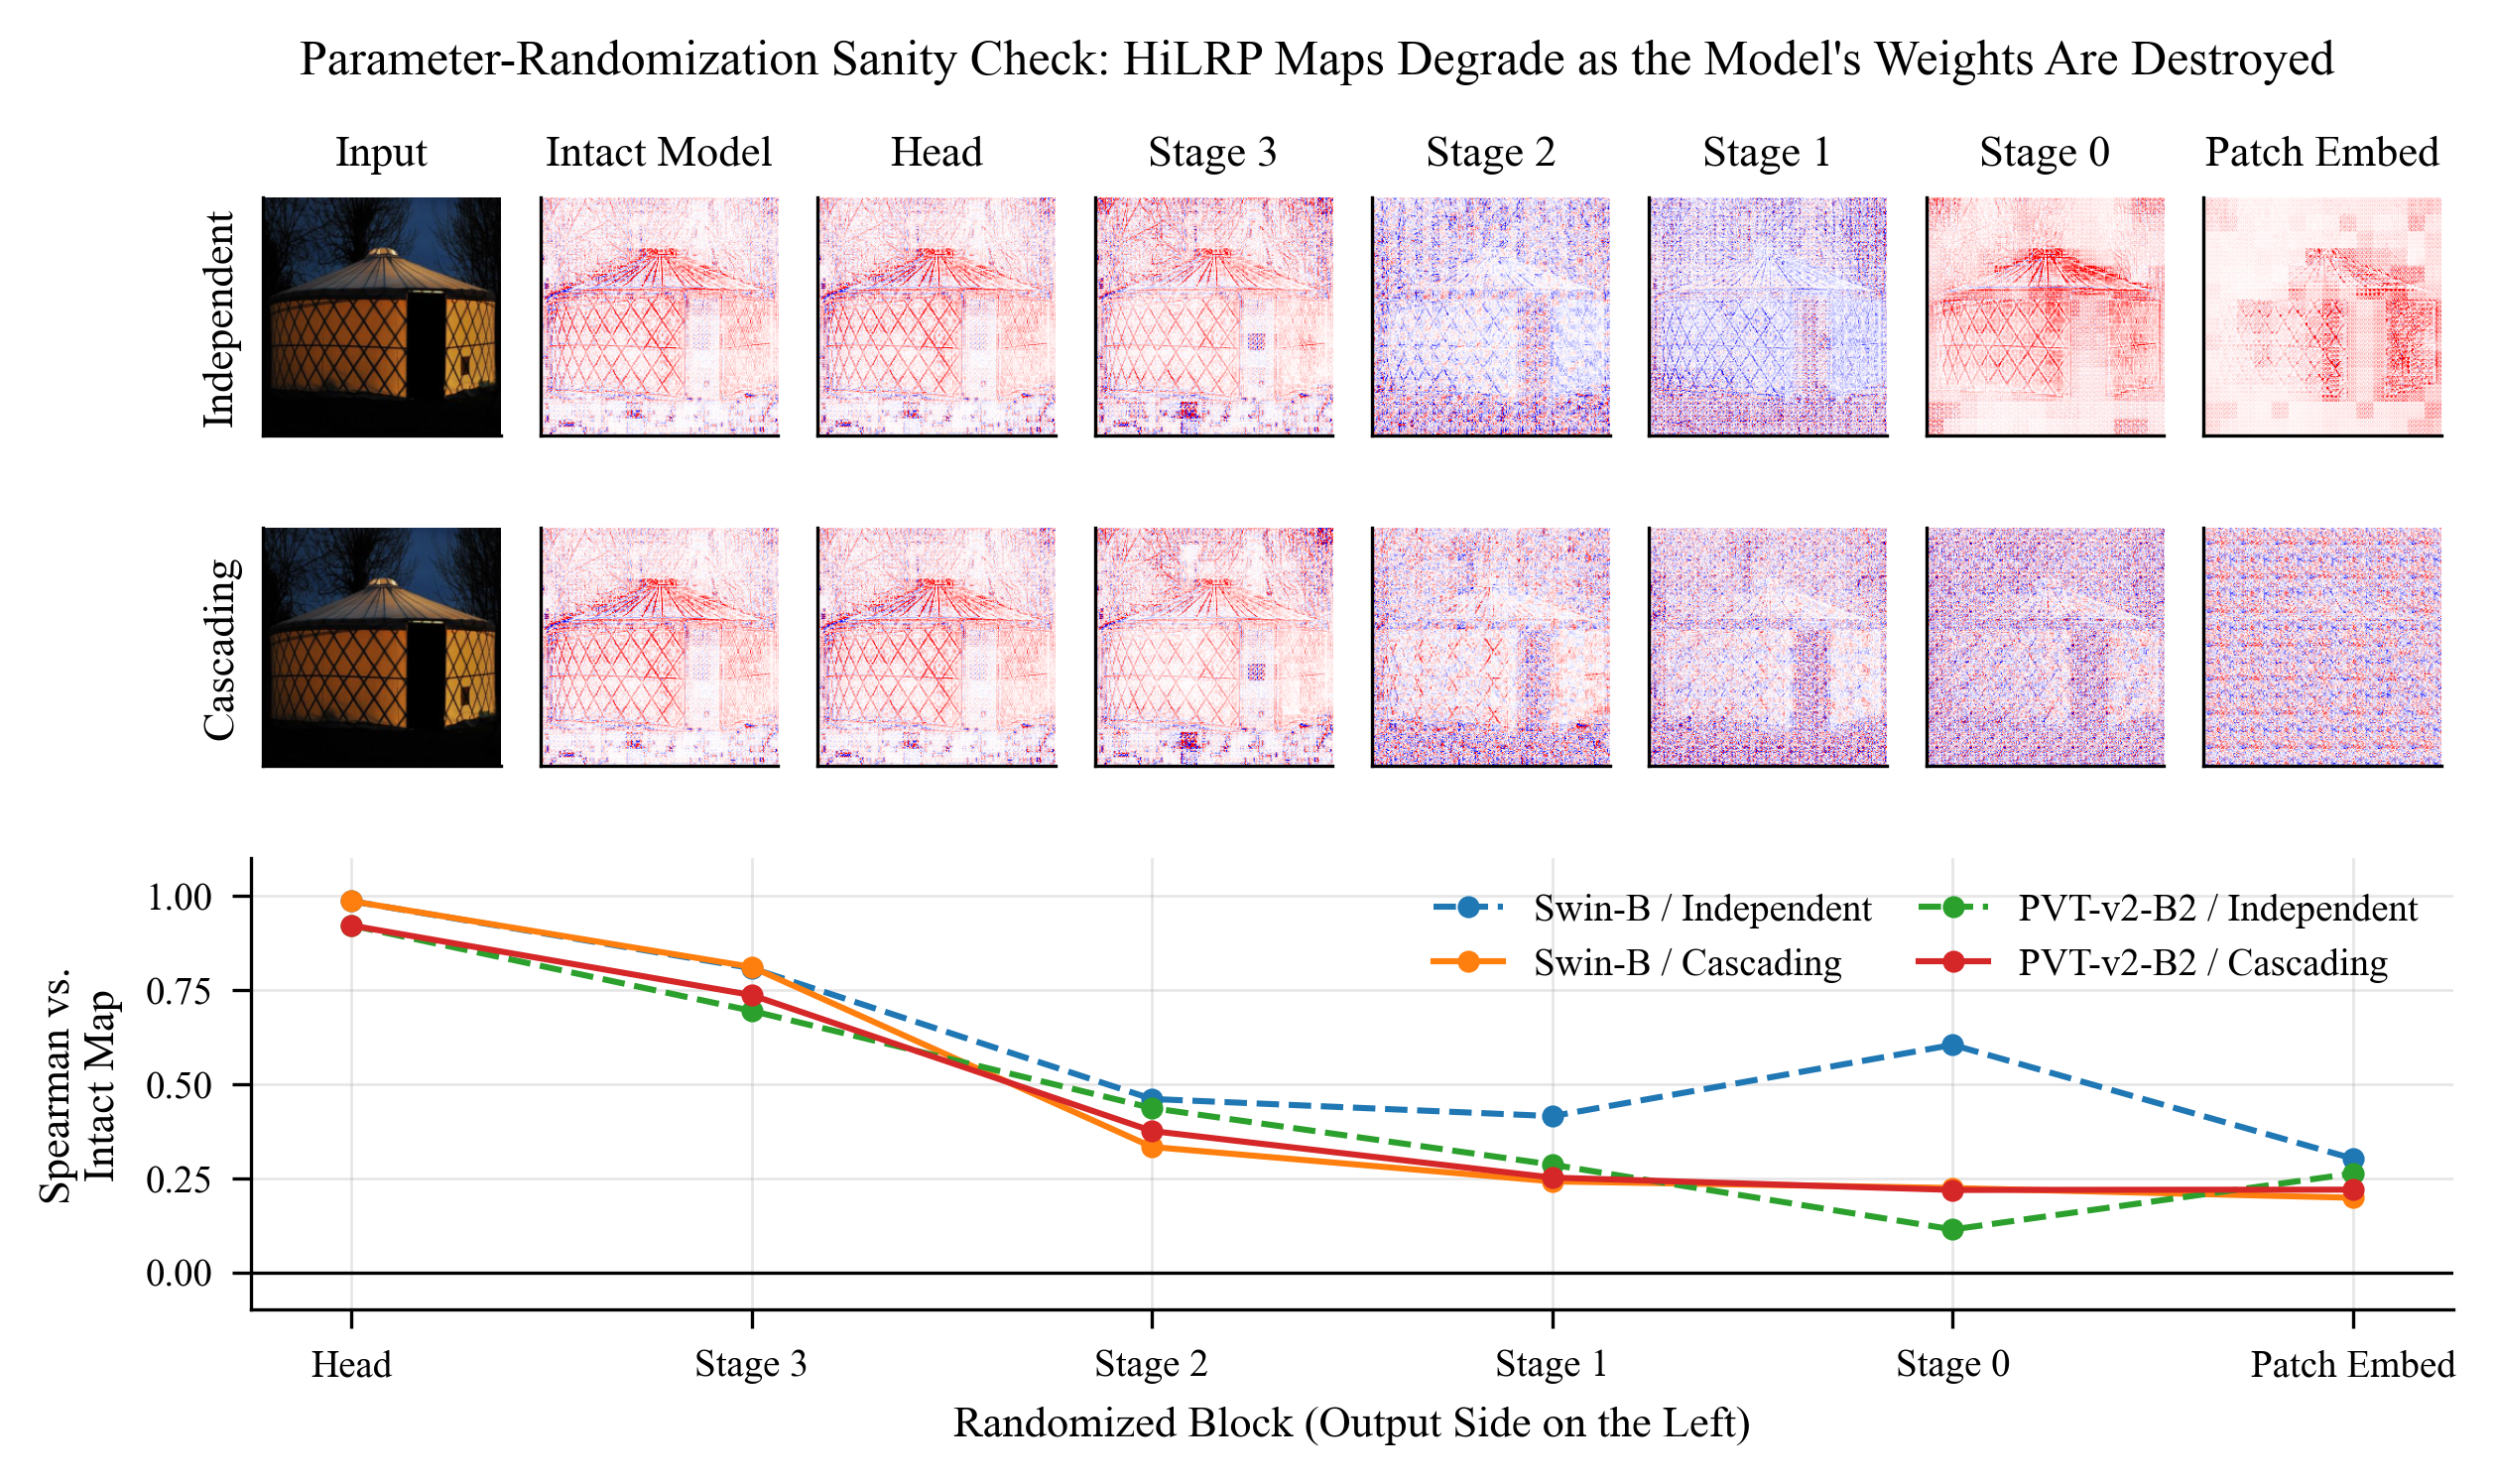
\includegraphics[width=\textwidth]{figures/hilrp/sanity_check.png}
  \caption{\textbf{HiLRP depends on the model's weights.} Top: independent
  randomization, in which one block is randomized and then restored. Middle:
  cascading randomization, in which blocks are randomized cumulatively from the
  output backwards. Bottom: agreement with the intact map against randomization
  depth for both protocols and backbones (solid cascading, dashed independent).}
  \label{fig:sanity}
\end{figure*}

\subsection{Convergence of the Shapley Reference}
\label{sec:shapley-convergence}
Because the Shapley agreement of Sec.~\ref{sec:shapley} is our primary evidence,
the sampling budget behind it needs to be justified rather than asserted.
Fig.~\ref{fig:shapley-convergence} runs the estimator to $m{=}128$ permutations
on Swin-T and reads the running estimate off the prefix of the same permutation
sequence, so the whole curve comes from one run.

Both curves settle before the budget we use. The reference agrees with its own
$m{=}128$ estimate at Spearman $0.969\pm0.016$ by $m{=}64$, against $0.593$ at
$m{=}4$, so the ranking of segments is essentially fixed by then. The reported
quantity converges sooner still: HiLRP's agreement is $0.627$ at $m{=}64$ and
$0.631$ at $m{=}128$, a difference of $0.004$ against a standard error of
$0.038$, so doubling the budget does not move the number. We therefore use
$m{=}64$ throughout. Absolute values here are computed on a $20$-image subset
and are not directly comparable with the $n{=}50$ scores of
Table~\ref{tab:shapley}; what this experiment establishes is the budget, not the
score.

\begin{figure}[!tbp]
  \centering
  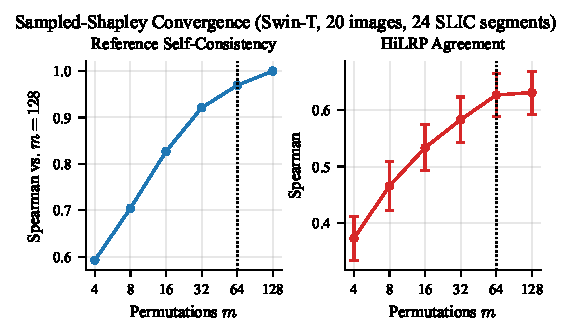
\includegraphics[width=\linewidth]{figures/hilrp/shapley_convergence.pdf}
  \caption{\textbf{The Shapley reference is converged at the budget we use.}
  Left: agreement of the estimate at $m$ permutations with the $m{=}128$
  estimate, measuring how settled the reference is. Right: HiLRP's agreement
  with the reference at each $m$, with standard errors. The dotted line marks
  $m{=}64$, past which both curves are flat. Swin-T, $20$ images, $24$ SLIC
  segments.}
  \label{fig:shapley-convergence}
\end{figure}

\subsection{Qualitative Results: Stage-Localized Relevance}
\label{sec:qualitative}
Figure~\ref{fig:qualitative} shows stage-localized relevance maps. Because relevance is conserved at every token-grid layer, the backward pass can be halted at an intermediate resolution stage ($28 \times 28$ or $14 \times 14$) and read out there. The maps move from high-resolution boundary structure in the early stages to compact, semantic object localization in the final $7 \times 7$ stage, showing where in the network the object representation is assembled.

Grad-CAM and the other CAM variants cannot produce this decomposition, because they attach to a single terminal spatial layer and upsample from it.

\subsection{Computational Cost}
\label{sec:cost}
HiLRP is a single forward and backward pass, so its cost is one gradient-order evaluation regardless of how many resolution stages are read out.
Table~\ref{tab:runtime} measures every method in the benchmark under the sameconfiguration the benchmark uses, on ViT-B/16 with one $224{\times}224$ image.
Costs are timed at batch size $1$, the worst case per image, and each method is timed \emph{before} HiLRP's process-global rule patches are installed, so no
baseline is measured through a patched forward.

The cost sits between two groups. Against the multi-pass methods HiLRP is cheaper on both axes: it is faster than the $20$-sample noise ensembles
(SmoothGrad, VarGrad, GradientSHAP, ${\approx}220$\,ms) while using a third of their memory ($0.97$ against $2.8$\,GB), $3\times$ faster than Integrated
Gradients, and one to two orders of magnitude faster than LIME, RISE, and
Occlusion, which need hundreds to thousands of forward passes. Against the
single-pass methods it is the expensive one: roughly $9\times$ the cost of
Grad-CAM ($21$\,ms) and $12\times$ that of Saliency ($16$\,ms), and its peak
memory is higher than either. The overhead is the rule-carrying forward and the
$\gamma$-composite, not extra passes. For a high-volume explanation pipeline
that difference is real, even though $0.2$\,s per image is small in absolute
terms.

One cost does not appear in the table. The stage-localized maps of
Fig.~\ref{fig:qualitative} come from the same backward pass, one relevance
capture per resolution stage, at no additional cost, whereas a per-stage
Grad-CAM requires a separate instrumentation point and a recomputation for each layer.

\begin{table}[!tbp]
  \centering
  \caption{\textbf{Cost per explanation.} ViT-B/16, one $224{\times}224$ image,
  batch size $1$, RTX~4070 Laptop. \emph{Passes} is the number of forward
  evaluations the method requires per explanation, which distinguishes the two
  groups. Methods are configured exactly as in the benchmark grid. Timings are
  the mean over repeated runs after warm-up; memory is peak allocated.}
  \label{tab:runtime}
  \setlength{\tabcolsep}{5pt}
  \footnotesize
  \begin{tabular}{@{}l r r r@{}}
    \toprule
    Method & Time (ms) \down & Peak mem.\ (GB) \down & Passes \\
    \midrule
    \multicolumn{4}{@{}l}{\emph{Single pass}} \\
    \quad Input$\times$Grad     & $15$ & $0.49$ & $1$ \\
    \quad Saliency              & $16$ & $0.49$ & $1$ \\
    \quad Attention Rollout     & $18$ & $0.52$ & $1$ \\
    \quad Grad-CAM              & $21$ & $0.72$ & $1$ \\
    \quad Grad-CAM++            & $21$ & $0.72$ & $1$ \\
    \quad \textbf{HiLRP (ours)} & $197$ & $0.97$ & $1$ \\
    \addlinespace
    \multicolumn{4}{@{}l}{\emph{Multi-pass}} \\
    \quad GradientSHAP          & $221$ & $2.83$ & $20$ \\
    \quad VarGrad               & $221$ & $2.81$ & $20$ \\
    \quad SmoothGrad            & $224$ & $2.81$ & $20$ \\
    \quad Integrated Gradients  & $588$ & $0.85$ & $50$ \\
    \quad LIME                  & $869$ & $0.38$ & $100$ \\
    \quad RISE                  & $2458$ & $1.55$ & $2000$ \\
    \quad Occlusion             & $5579$ & $0.38$ & $784$ \\
    \bottomrule
  \end{tabular}
\end{table}

\begin{figure*}[!tbp]
  \centering
  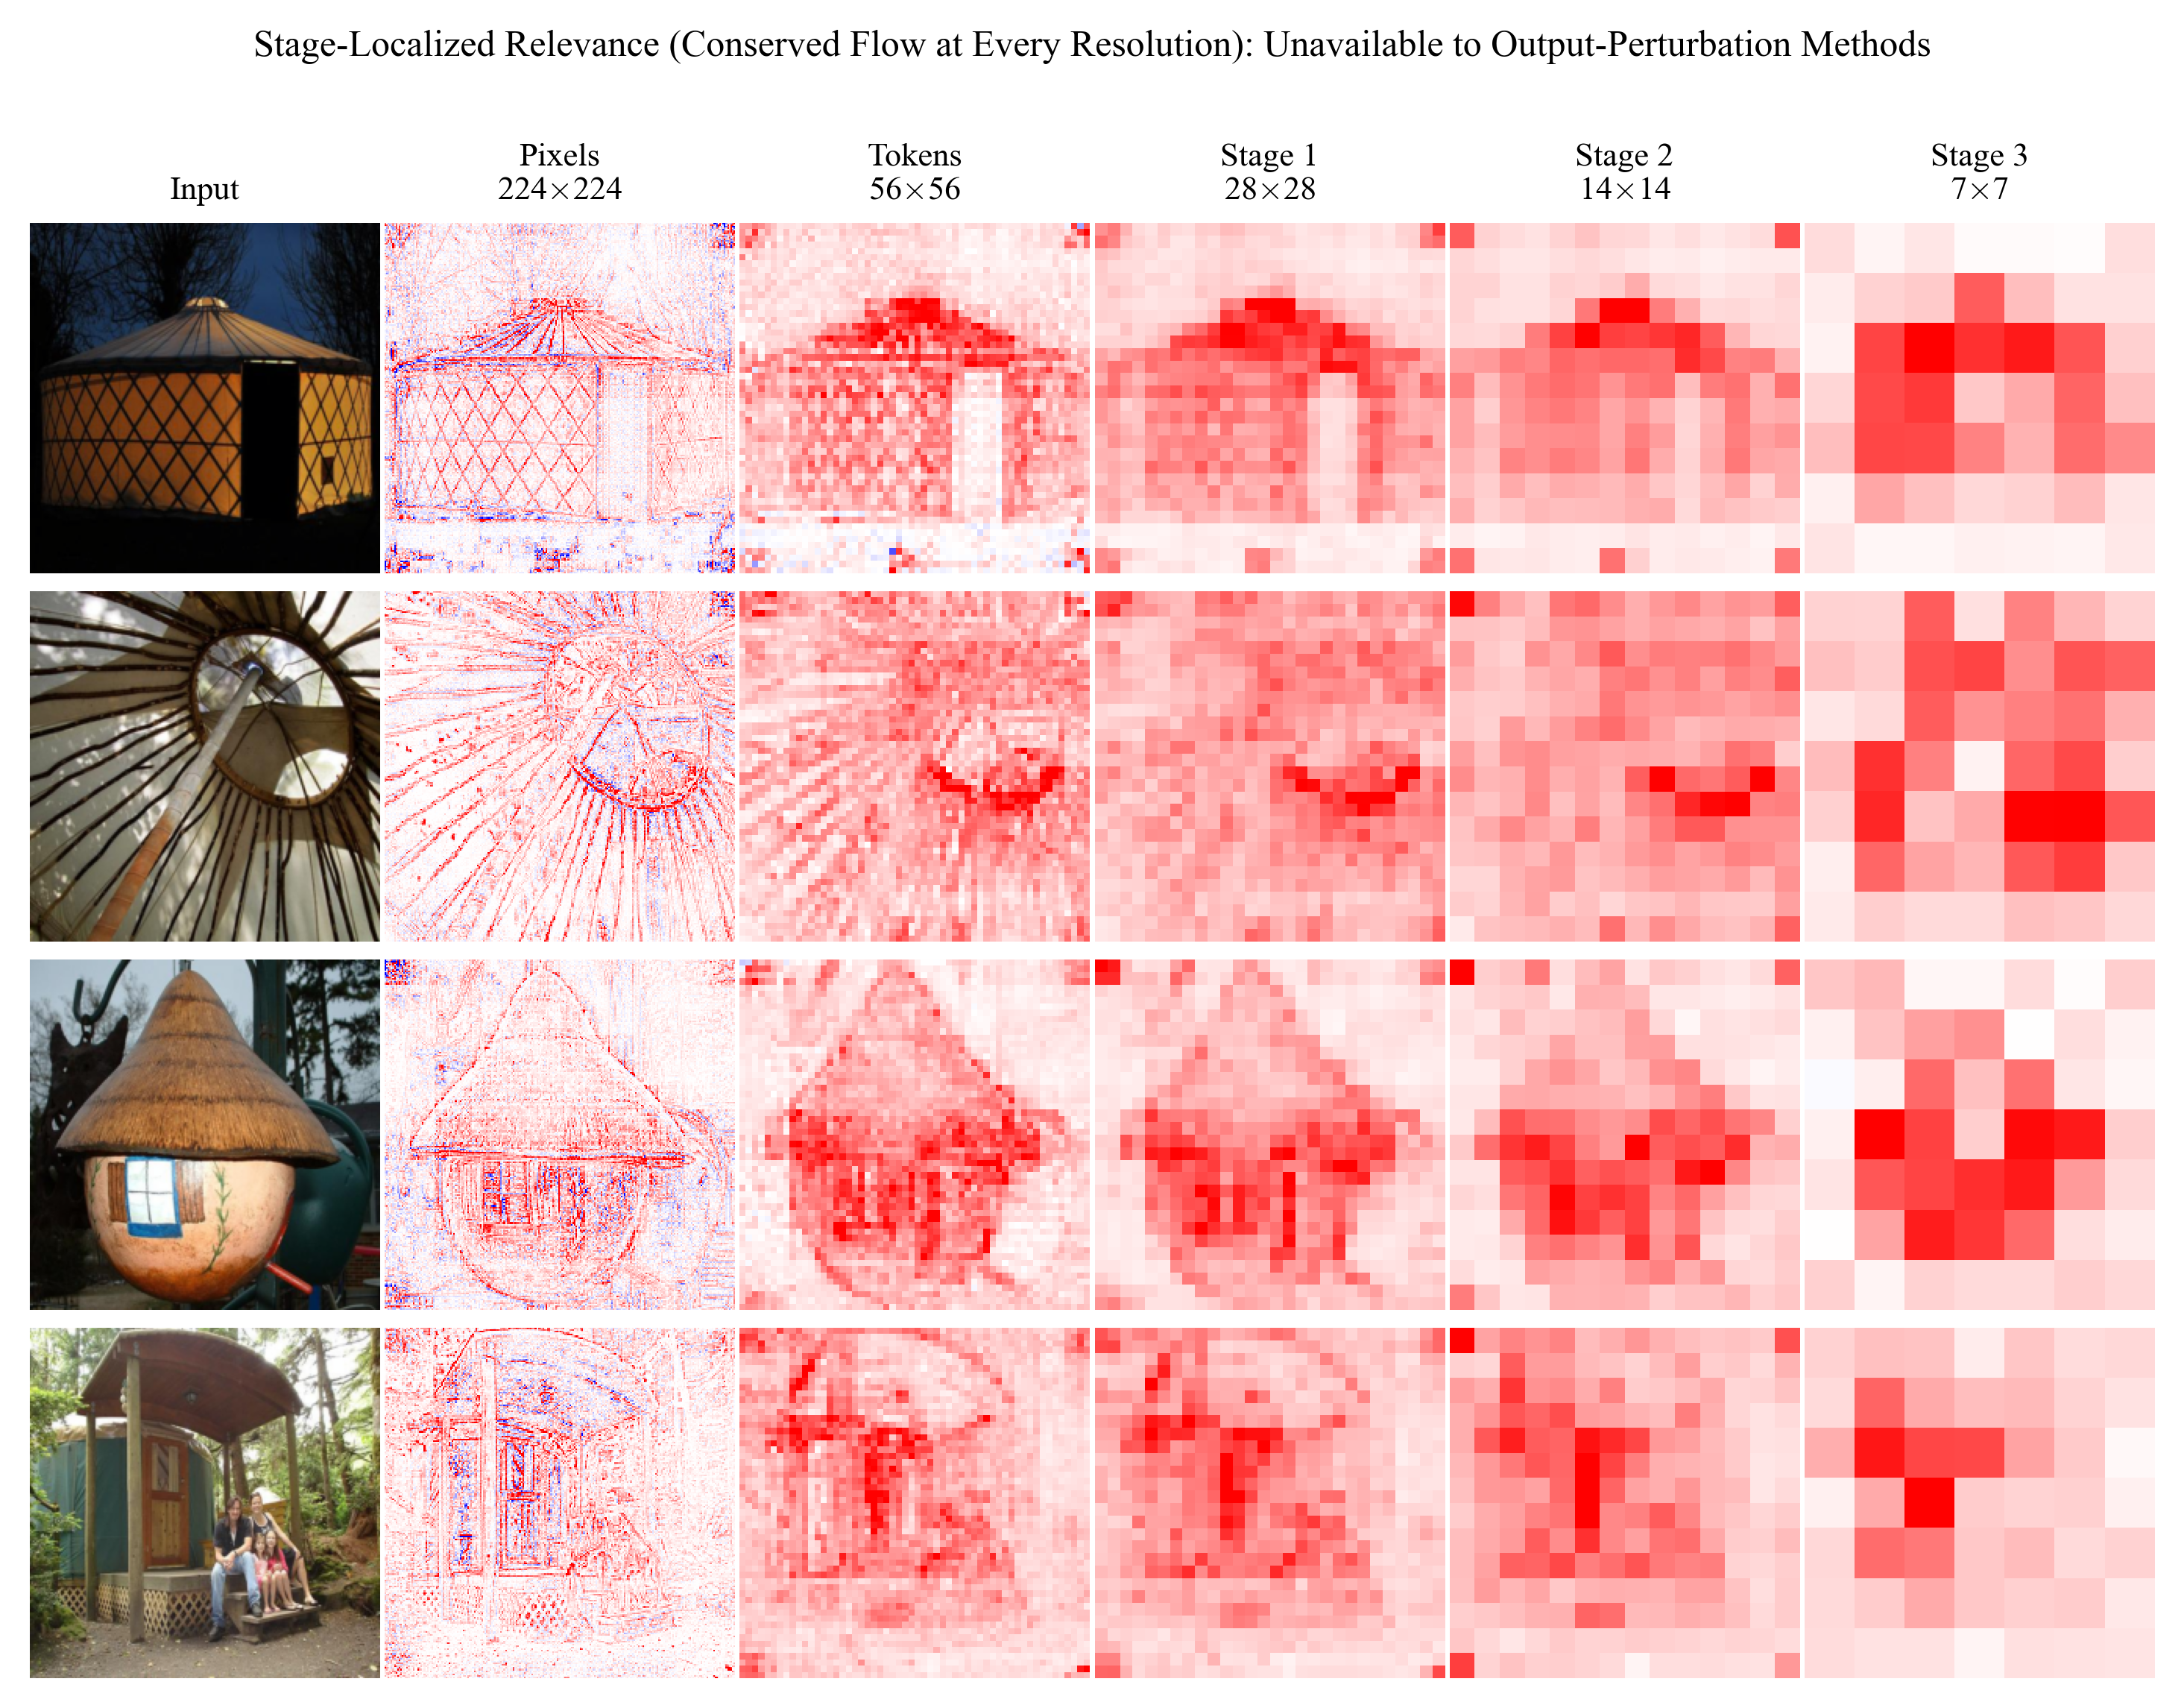
\includegraphics[width=\textwidth]{figures/hilrp/stage_localization.png}
  \caption{\textbf{Stage-localized relevance on Swin-B.} The backward pass is
  halted at each resolution stage and read out: input pixels ($224$), the token
  grid ($56$), and the merged stages ($28,14,7$).}
  \label{fig:qualitative}
\end{figure*}

\subsection{The Pretraining Objective, Not the Architecture, Determines Explanation Structure}
\label{sec:rq2}
A conservation-based, label-free attributor can explain a model \emph{in its own representational objective}, rather than through a bolted-on linear probe that would replace every model's objective with a shared classifier. We use this to ask whether the pretraining objective, and not the architecture, shapes what a model finds explanatory. We fix the backbone family (ViT-B) and vary pretraining at six public checkpoints: supervised (AugReg), DINO, DINOv2, DINOv2 with registers, MAE, and CLIP. Each is attributed under one common label-free scalar, the view-invariance similarity $s=\cos(g(x),g(x'))$ between a horizontal-flip pair, on identical inputs. The supervised, DINO, MAE, and CLIP checkpoints share the ViT-B/16 layout ($197{\times}768$ tokens); the two DINOv2 variants are ViT-B/14 at $224$\,px. Holding the scalar, the inputs, and the backbone family fixed leaves the pretraining objective as the varying factor.

Table~\ref{tab:rq2} reports the results over 30 images. The six objectives produce structurally different explanations: the mean pairwise Spearman agreement of their maps is $0.36$, far from the $1.0$ that would hold if the objective were irrelevant, and MAE is the strongest outlier ($0.19$--$0.32$ agreement with the others). The differences line up with known representational properties. The DINO family localizes best: DINO, DINOv2, and DINOv2 with registers all reach label-free Pointing $0.97$, recovering the objective's documented emergent object-centricity across two model generations without using any label. DINOv2 reaches this localization while routing about half as much relevance mass to the pixels as DINO ($0.27$ against $0.51$), and adding the four register tokens changes the map only mildly (agreement $0.50$ between the two DINOv2 variants). MAE routes almost no relevance to the input pixels ($0.07$ of the scalar), consistent with a reconstruction objective whose \textsc{cls} embedding is not organized for view invariance, and CLIP's evidence is the least object-localized ($0.40$). The maps show the same pattern (Fig.~\ref{fig:rq2-maps}). We frame this as exploratory. There is no ground truth for the ``correct'' view-invariance map, so we report the structural differences between objectives and their consistency with documented properties (DINO's emergent object-centricity, MAE's reconstruction organization), not a correctness claim about any single map.

\begin{table}[!tbp]
  \centering
  \caption{\textbf{Pretraining objective and explanation structure.} One common
  label-free scalar attributed across six pretraining objectives on frozen ViT-B
  backbones; the DINOv2 variants are ViT-B/14 at $224$\,px. \emph{View sim.}\ is
  the attributed scalar $s$ of Eq.~\eqref{eq:view-sim}, averaged over images;
  \emph{Label-free point} is the Pointing Game on the map produced from $s$;
  \emph{Pixel-rel.}\ is the fraction $\sum_i R_i/s$ reaching the input pixels.}
  \label{tab:rq2}
  \setlength{\tabcolsep}{5pt}
  \resizebox{\columnwidth}{!}{%
  \begin{tabular}{l c c c}
    \toprule
    Objective & View sim.\ $s$ & Label-free point & Pixel-rel. \\
    \midrule
    Supervised  & 0.972 & 0.60 & 0.57 \\
    DINO        & 0.993 & \textbf{0.97} & 0.51 \\
    DINOv2      & 0.980 & \textbf{0.97} & 0.27 \\
    DINOv2-reg4 & 0.982 & \textbf{0.97} & 0.29 \\
    MAE         & 0.999 & 0.47 & \textbf{0.07} \\
    CLIP        & 0.977 & 0.40 & 0.39 \\
    \midrule
    \multicolumn{4}{l}{\footnotesize Mean pairwise map agreement (Spearman): $\mathbf{0.36}$ (vs.\ $1.0$ if objective-invariant)} \\
    \bottomrule
  \end{tabular}%
  }
\end{table}

\begin{figure*}[!tbp]
  \centering
  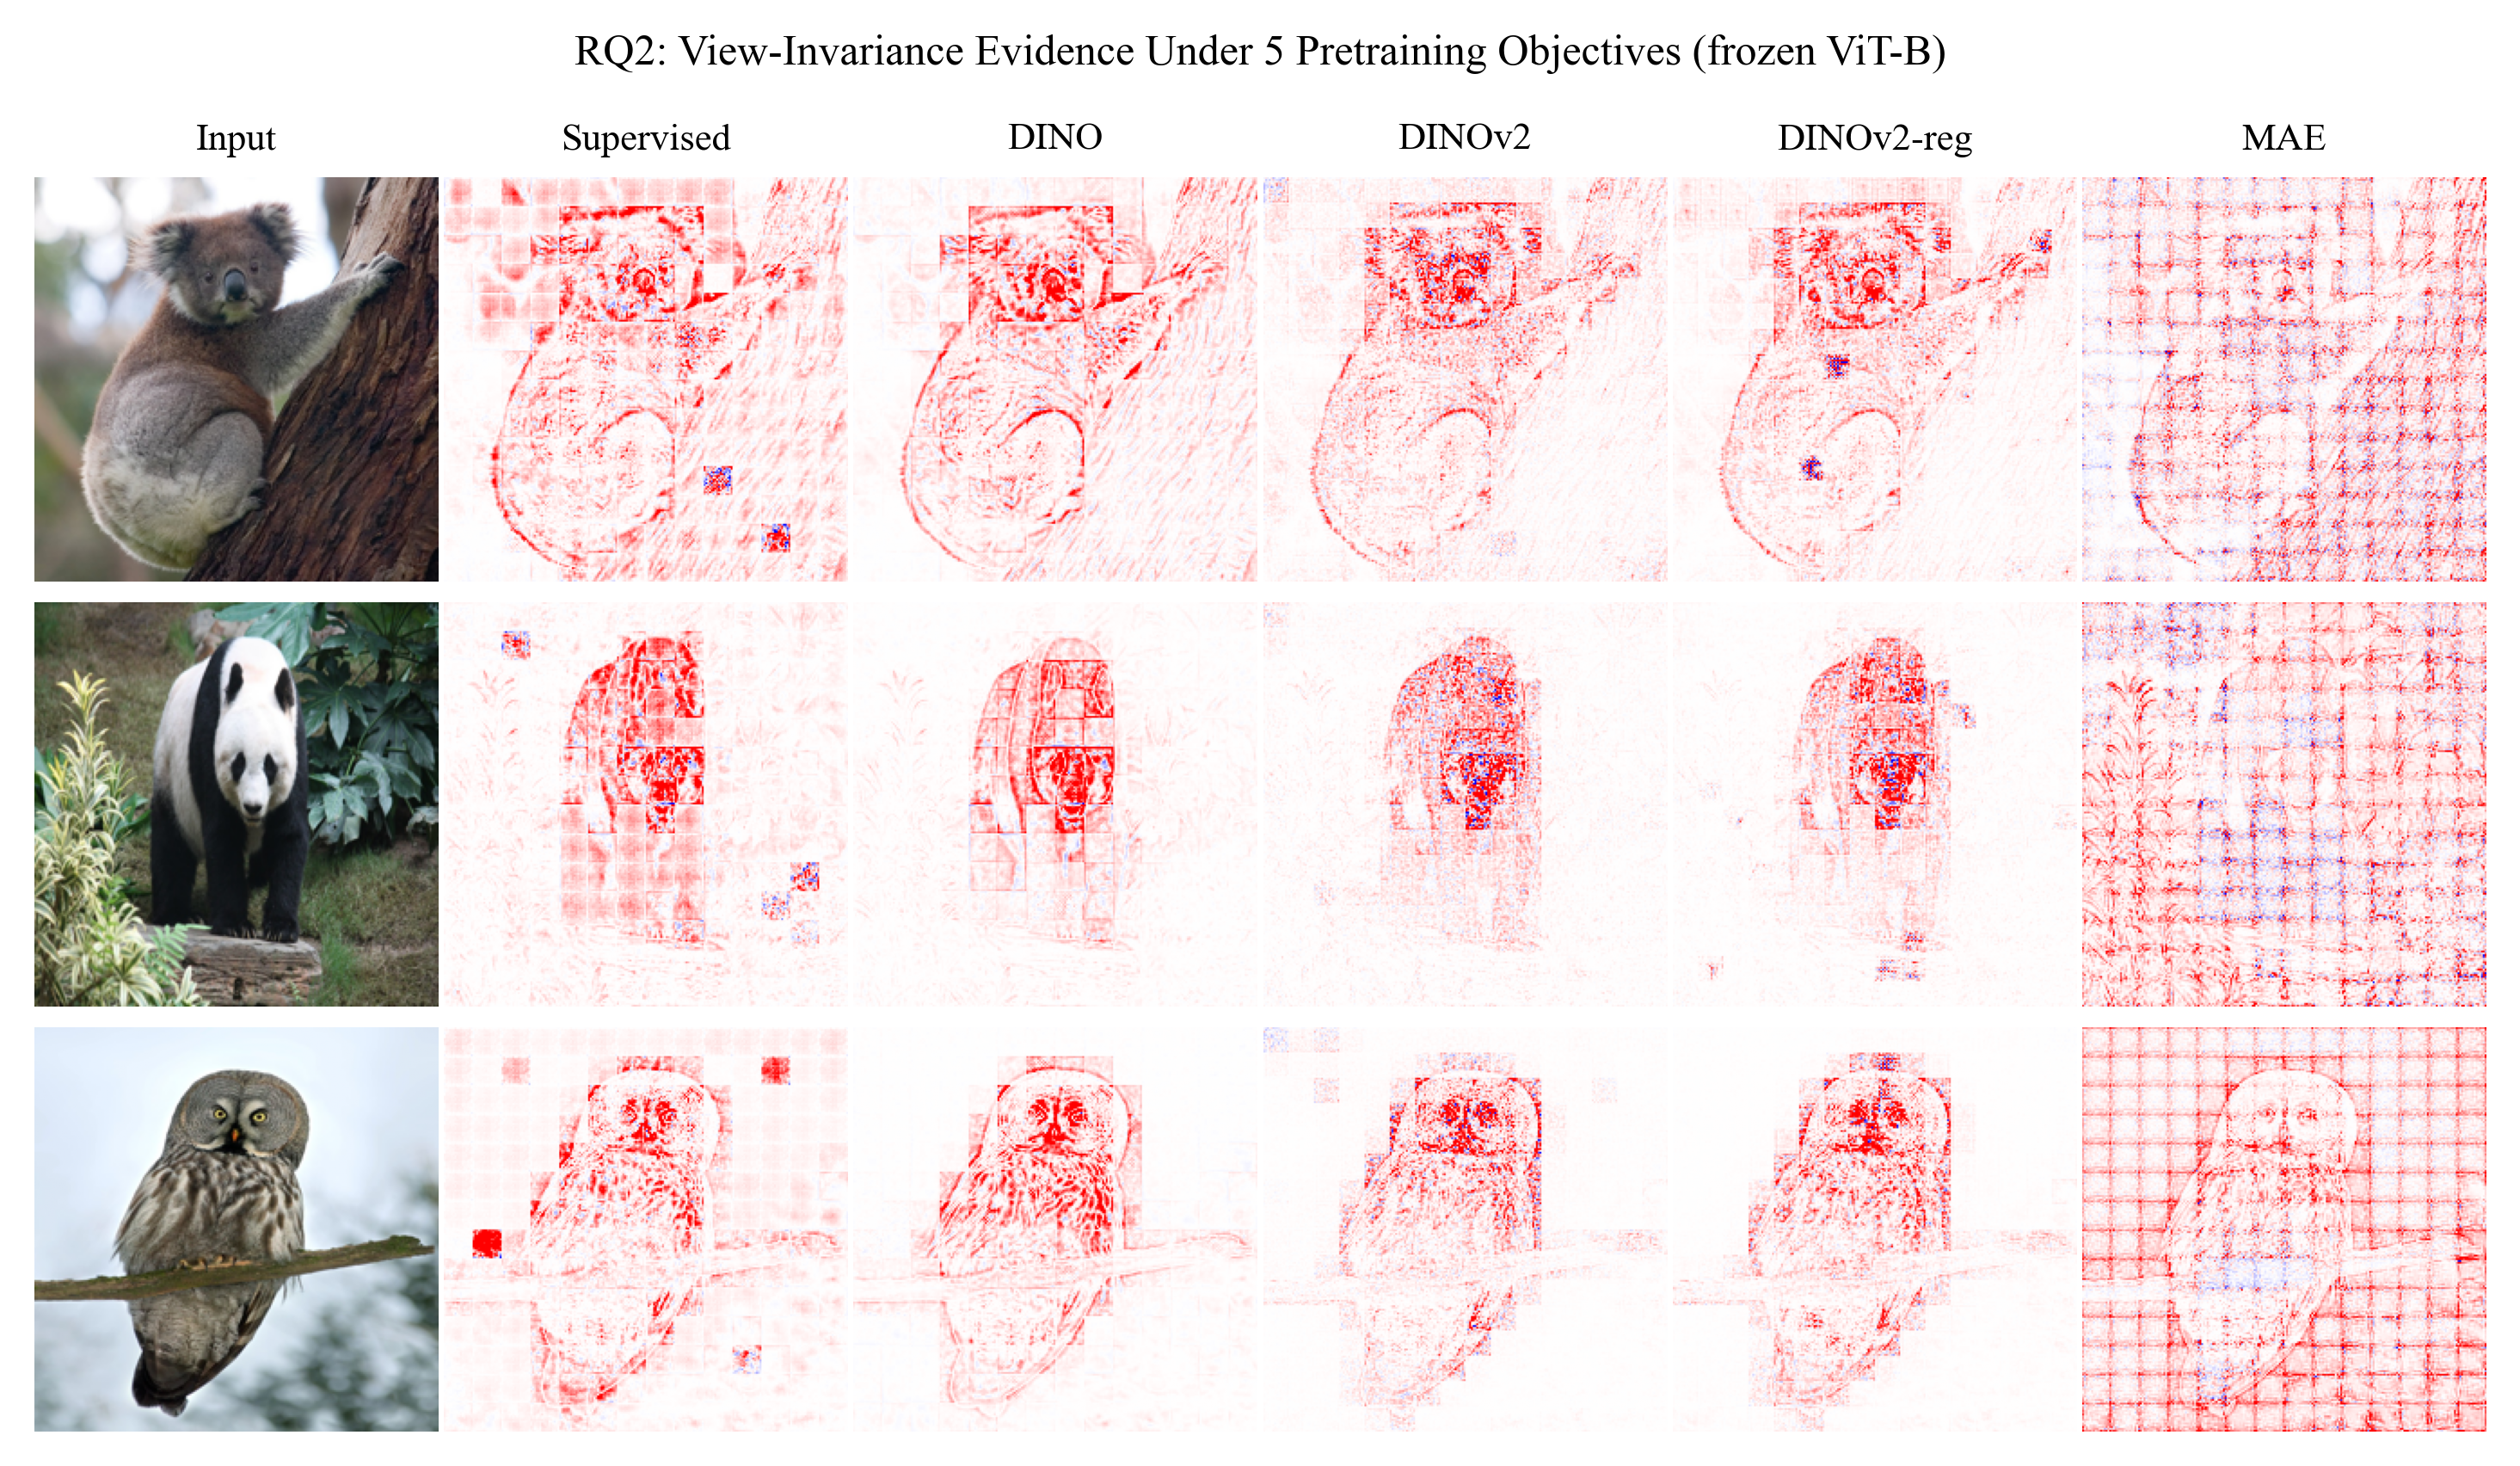
\includegraphics[width=\textwidth]{figures/hilrp/rq2_maps.png}
  \caption{\textbf{Label-free attribution.} The same view-invariance scalar attributed across five frozen ViT-B pretraining objectives on clean single-object images. The maps differ structurally: the DINO family traces object structure, while MAE shows the reconstruction patch grid rather than the object. CLIP is attributed separately in Fig.~\ref{fig:clip}.}
  \label{fig:rq2-maps}
\end{figure*}

\subsection{Cross-Attention and Multi-Modal Attribution}
\label{sec:multimodal}
Cross-attention, where queries from one stream attend to keys and values from another, is the mechanism prior transformer LRP handles least, yet it is a direct instance of the bilinear and softmax primitives with two input streams. CrossViT realizes it inside a classification ViT: the class token of each token-scale branch attends to the other branch's tokens through six cross-attention blocks. HiLRP applies the same CP-LRP rule to the branch self-attention and to the cross-attention. The patched model is forward-equivalent to the original (maximum absolute logit deviation $<10^{-6}$) and attains a Pointing score of $0.980$, matching the best backbone in Table~\ref{tab:bigbench} on a two-branch design for which attention rollout has no single path to follow.

The scalar being explained need not even come from a single modality. On CLIP
(ViT-B/16), let
$f_{\text{img}}:\mathbb{R}^{H\times W_{\mathrm{img}}\times 3}\to\mathbb{R}^{d}$
be the frozen image tower, which embeds an image into the $d$-dimensional joint
image-text space, and let $f_{\text{text}}:\mathcal{T}\to\mathbb{R}^{d}$ be the
frozen text tower, which embeds a tokenized caption $t\in\mathcal{T}$ into the
same space. We attribute the image-text alignment
\begin{equation}
\label{eq:clip-sim}
s \;=\; \cos\!\big(f_{\text{img}}(x),\,f_{\text{text}}(t)\big),
\end{equation}
in which the caption $t$ is held fixed, so no gradient flows through
$f_{\text{text}}$ and the attribution is delivered entirely to the pixels of
$x$. HiLRP then answers what image evidence supports a given textual
description. The patched image tower is forward-equivalent to the original (maximum absolute deviation $<10^{-6}$), and the attribution is text-conditioned (Fig.~\ref{fig:clip}): on clean single-object images the caption that matches the image scores a higher similarity than an unrelated caption ($0.33$ against $0.20$ for the koala, $0.32$ against $0.19$ for the panda, $0.31$ against $0.20$ for the owl) and concentrates more positive relevance on the object. We present this as a qualitative demonstration rather than a quantitative localization claim, since CLIP's evidence is diffuse (its label-free localization is the weakest in Table~\ref{tab:rq2}). It exercises the cross-modal scalar and the multi-head attention primitive on a pretrained multi-modal model with no new rule, extending conservation-based attribution beyond the single-model, single-label setting of prior transformer LRP.

\begin{figure}[!tbp]
  \centering
  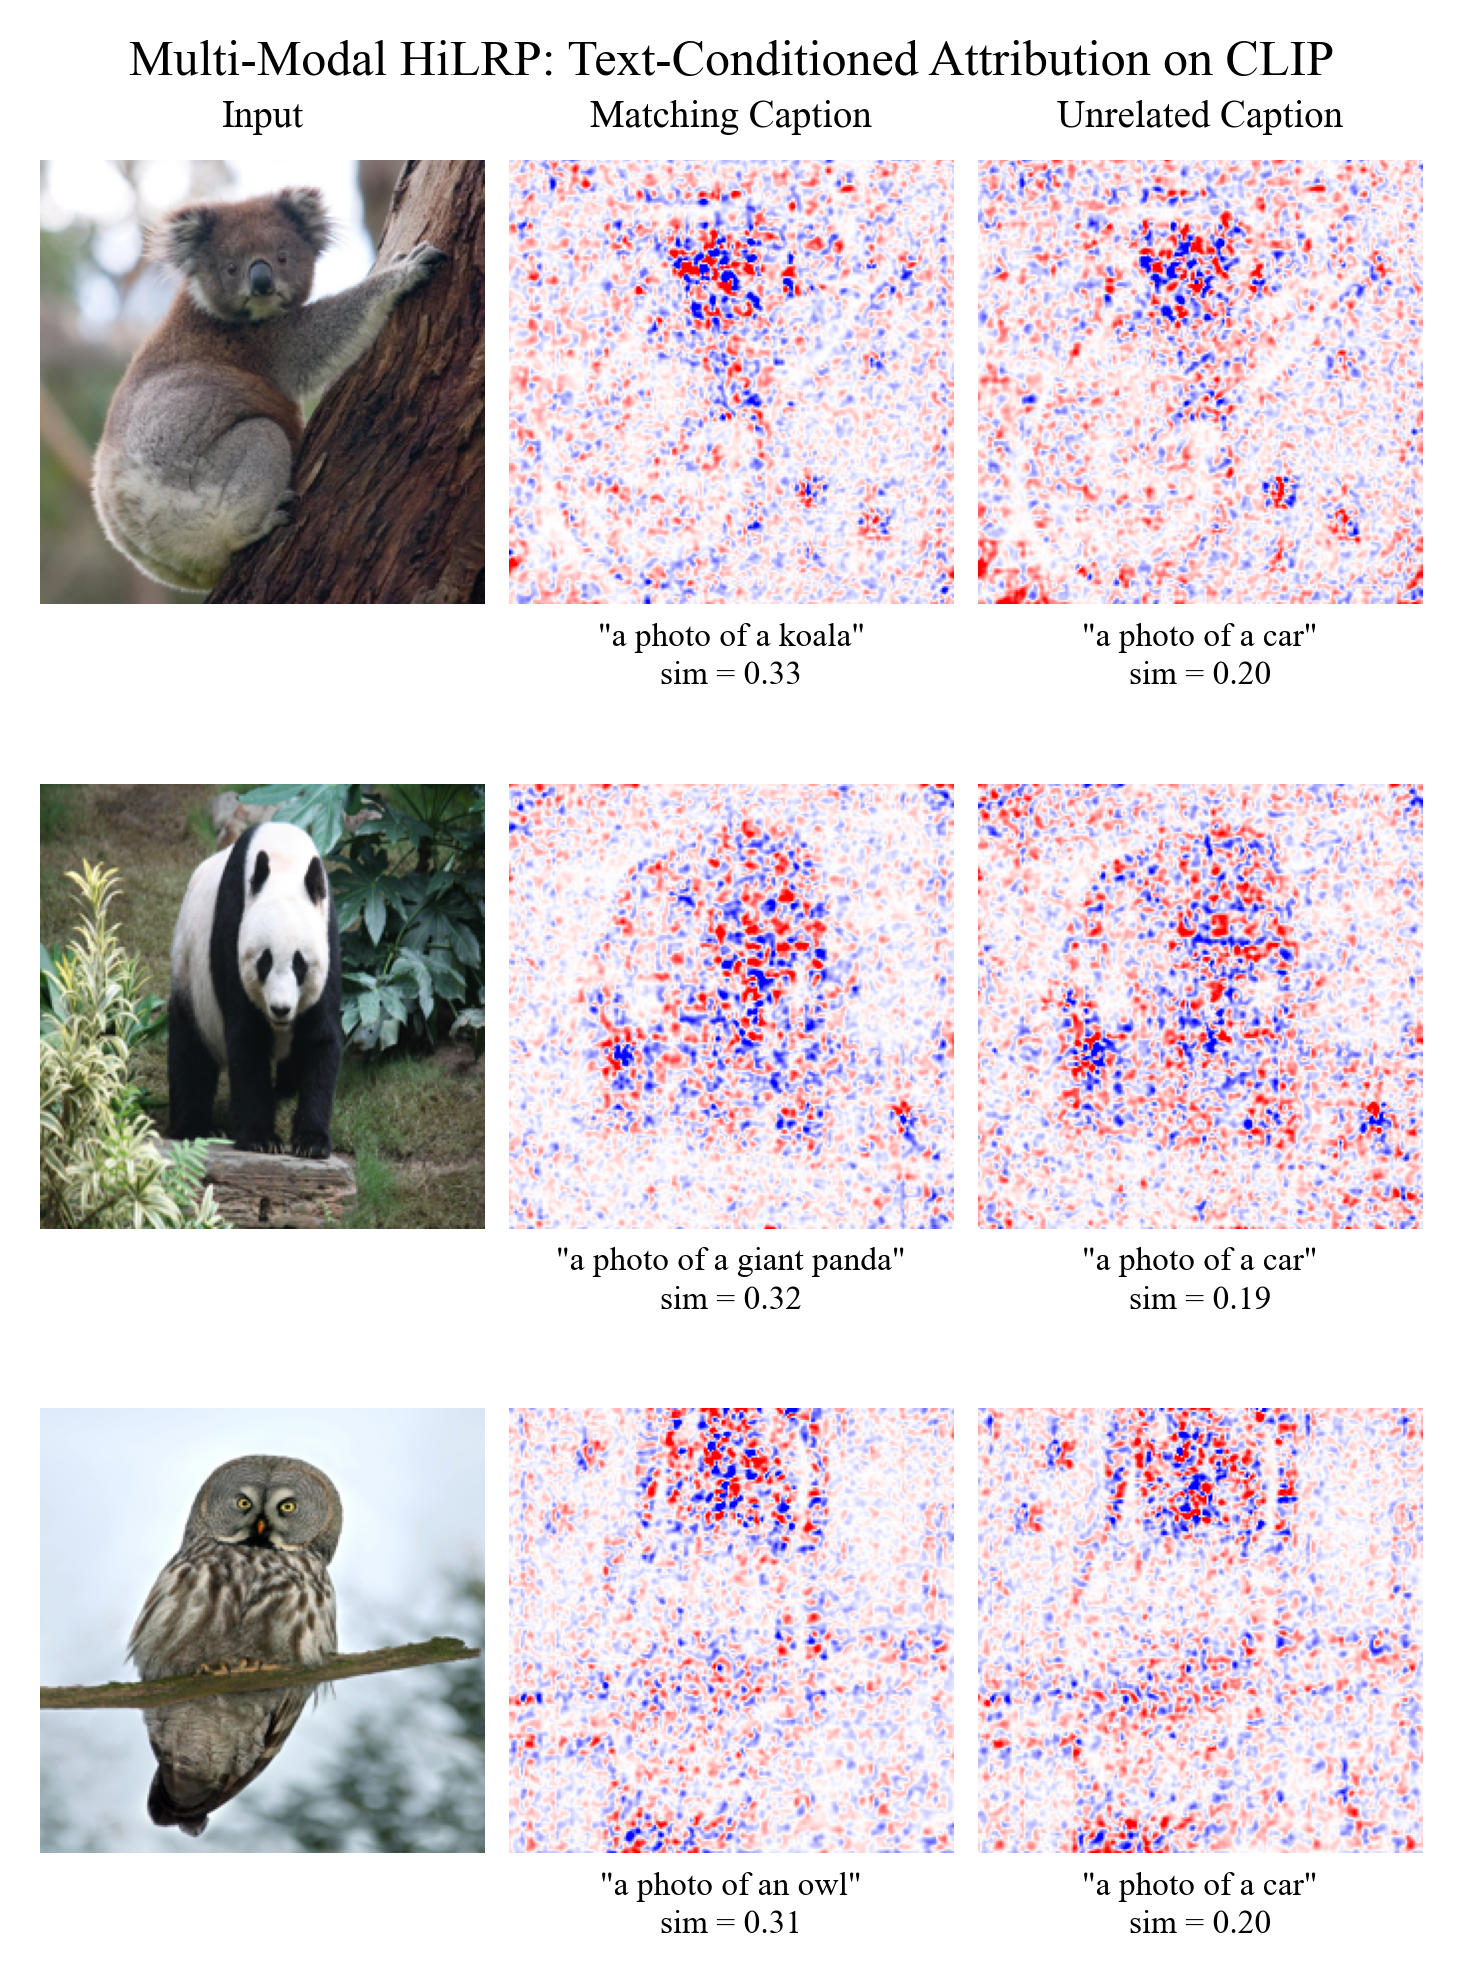
\includegraphics[width=\linewidth]{figures/hilrp/clip_multimodal.png}
  \caption{\textbf{Text-conditioned multi-modal attribution on CLIP.} HiLRP
  attributes the image-text similarity of Eq.~\eqref{eq:clip-sim} on CLIP
  ViT-B/16 with the caption held frozen, for a matching caption
  (\emph{``a photo of a koala/giant panda/owl''}) and an unrelated one
  (\emph{``a photo of a car''}).}
  \label{fig:clip}
\end{figure}

\subsection{Ablation of the Relevance-Rule Choices}
\label{sec:ablation}
Table~\ref{tab:ablation} isolates HiLRP's two relevance-rule decisions on Swin-B: the attention rule and the $\gamma$ schedule. Two primary observations emerge. First, conservation holds under \emph{every} configuration (error ${\approx}0.02$), so on this backbone conservation validity is a property of the construction rather than of a tuned setting, and the choices affect \emph{localization} only. This also holds on PVT-v2, but not on the linear-attention family, where $\gamma$ additionally governs a relevance inflation (Sec.~\ref{sec:gamma}). Second, the $\gamma$-rule has a substantial effect: the pure-$\epsilon$ limit ($\gamma{=}0$) reduces Pointing to $0.56$ despite conserving relevance, while $\gamma{=}0.25$ restores it to $0.955$. On Swin the two attention rules are within noise of each other ($0.955$ against $0.950$); CP-LRP is the default because of its conservation advantage on the other hierarchical backbones (Sec.~\ref{sec:conservation-validity}), not because of this margin. The selection principle for $\gamma$ follows from the same structure: conservation holds for every $\gamma$, so we pick the value that maximizes localization under that constraint and keep it global at $\gamma{=}0.25$ rather than tuning per architecture. Localization is non-increasing in $\gamma$ on EfficientViT, so $0.25$ is a conservative global setting. An adaptive per-layer schedule is left to future work.

\begin{table}[!tbp]
  \centering
  \caption{\textbf{Ablation of HiLRP's relevance-rule choices} on Swin-B ($n{=}200$ ImageNet-S). \textsc{Pointing} measures localization (higher is better); \textsc{Cons.\ err.}\ is the mean conservation error $|\sum_i R_i / f_c(x)-1|$ (lower is better). Conservation holds ($\approx0.02$) under every choice \emph{by construction}; the rule choices tune localization only. Pure $\epsilon$ ($\gamma{=}0$) conserves yet substantially reduces localization. Best per column in bold.}
  \label{tab:ablation}
  \setlength{\tabcolsep}{6pt}
  \begin{tabular}{l cc}
    \toprule
    Configuration & Pointing $\uparrow$ & Cons.\ err.\ $\downarrow$ \\
    \midrule
    \multicolumn{3}{l}{\emph{1) Attention relevance rule} ($\gamma{=}0.25$)} \\
    \quad AttnLRP-through           & 0.950 & 0.019 \\
    \quad CP-LRP (ours)             & \textbf{0.955} & 0.019 \\
    \addlinespace
    \multicolumn{3}{l}{\emph{2) $\gamma$ schedule} (attention $=$ CP-LRP)} \\
    \quad $\gamma{=}0$ (pure $\epsilon$) & 0.560 & 0.022 \\
    \quad $\gamma{=}0.25$ (ours)     & \textbf{0.955} & 0.019 \\
    \quad $\gamma{=}0.5$             & 0.950 & \textbf{0.018} \\
    \midrule
    \textbf{HiLRP (full: CP-LRP, $\gamma{=}0.25$)} & \textbf{0.955} & 0.019 \\
    \bottomrule
  \end{tabular}
\end{table}

\subsection{Selection of the  \texorpdfstring{$\gamma$}{gamma} Parameter}
\label{sec:gamma}
The $\gamma$-rule on linear and convolutional layers is HiLRP's main hyperparameter. As $\gamma\to0$ it recovers the pure $\epsilon$-rule, exact in conservation but noisier at the pixel level; larger $\gamma$ emphasizes positive evidence, denoising the map at the cost of a bias toward positive contributions. Table~\ref{tab:gamma} sweeps $\gamma$ over $100$ images, applying it uniformly to the linear and convolutional layers, and reports both Pointing and the head-adjacent relevance sum.

The evaluation across $\gamma$ values reveals two distinct regimes, which delineates the exact bounds of the conservation guarantee. On Swin and 
PVT-v2 the relevance sum sits at $1.00$--$1.01$ for \emph{every} $\gamma$,
including the pure $\epsilon$ limit, so on those families $\gamma$ tunes
localization alone and conservation is a property of the construction rather
than of the setting. There $\gamma{=}0$ reduces Pointing sharply (to $0.66$ on Swin
and $0.85$ on PVT) while conserving perfectly, which is the cleanest statement
that conservation and localization are separate axes. EfficientViT-B2 behaves
differently: its head-adjacent sum is strongly $\gamma$-dependent, inflating
almost $13\times$ at $\gamma{=}0$ and falling monotonically to $0.99$ at
$\gamma{=}1.0$, while Pointing drifts down only slightly ($0.99$ to $0.95$). On
linear attention, therefore, $\gamma$ is critical for conservation as well
as for localization, and the claim that conservation is setting-independent
holds for the windowed and spatial-reduction families but not for this one. This
result is reported rather than omitted by restricting the sweep to the backbones
on which the simpler statement holds.

Absolute values in this sweep are not directly comparable with those of
Tables~\ref{tab:bigbench} and~\ref{tab:ablation}, since the sweep uses a
different image subset and applies $\gamma$ to the convolutional layers as well;
the Swin $\gamma{=}0$ entry reads $0.66$ here against $0.56$ in
Table~\ref{tab:ablation}. Only the trend across $\gamma$ should be read from the
table. We fix $\gamma{=}0.25$ on the linear and attention layers for all models and all experiments. The one refinement is a lower convolutional stabilizer, $\gamma_{\text{conv}}{=}0.05$, on the deep convolutional stack of the EfficientViT family: the global $0.25$ leaves head conservation intact but over-concentrates on positive contributions and zeroes the \emph{input-level} relevance there, whereas $0.05$ restores it at no cost to localization (Sec.~\ref{sec:conservation-validity}). This two-level default needs no per-image or per-model search beyond that single convolution-family setting.

\begin{table}[!tbp]
  \centering
  \caption{\textbf{Sensitivity to $\gamma$} ($n{=}100$ ImageNet-S images).
  Each cell reports Pointing\,/\,head-adjacent relevance sum, where $1.00$
  denotes exact conservation and $\gamma{=}0$ is the pure $\epsilon$ limit. Here
  $\gamma$ is applied uniformly to the linear and convolutional layers, which
  differs from the deployed EfficientViT configuration
  (Sec.~\ref{sec:implementation}).}
  \label{tab:gamma}
  \setlength{\tabcolsep}{3pt}
  \scriptsize
  \begin{tabular}{l ccccc}
    \toprule
    Backbone & $\gamma{=}0$ & $\gamma{=}0.1$ & $\bm{\gamma{=}0.25}$ & $\gamma{=}0.5$ & $\gamma{=}1.0$ \\
    \midrule
    Swin-B          & 0.66\,/\,1.00 & 0.96\,/\,1.00 & \textbf{0.99}\,/\,1.00 & 0.99\,/\,1.00 & 0.99\,/\,1.00 \\
    PVT-v2          & 0.85\,/\,1.01 & 0.98\,/\,1.01 & \textbf{0.97}\,/\,1.01 & 0.97\,/\,1.01 & 0.97\,/\,1.01 \\
    EfficientViT-B2 & 0.99\,/\,12.95 & 0.99\,/\,8.73 & \textbf{0.97}\,/\,4.35 & 0.96\,/\,2.17 & 0.95\,/\,0.99 \\
    \bottomrule
  \end{tabular}
\end{table}

\section{Limitations}
\label{sec:limitations}
Throughout this section, $x$ is the input image, $f_c(x)$ the logit of the explained class $c$, $R_i$ the relevance assigned to input element $i$, and $\gamma$ the stabilizer of the propagation rule in Eq.~\eqref{eq:gamma-rule}.

\textbf{Pixel-level conservation is approximate.} Conservation is exact at the token level through the proven operations (verified to $10^{-16}$), but the $\gamma$-rule applied to the patch-embedding and hybrid convolutional stem introduces a controlled deviation at the input-pixel level. The measured relevance-to-logit ratio at the pixels, $\sum_i R_i/f_c(x)$, ranges from $0.16$ to $0.77$ on Swin, PVT, and MaxViT, and is $0.13$ and $0.35$ on EfficientViT-B1 and B2 once their deep convolutional stack is stabilized with $\gamma_{\text{conv}}{=}0.05$ (the global $0.25$ zeroes it). We therefore state conservation as a token-level guarantee plus a quantified pixel-level deviation, never as end-to-end pixel exactness.

\textbf{MobileViT-v2 and the extension to globally-normalized hybrids.} MobileViT-v2's separable-attention block decomposes into the four primitives and is realized on the pretrained model (Table~\ref{tab:attn-coverage}), but the backbone around it is a structural outlier: depthwise separable convolutions, a single-group \textsc{GroupNorm} that normalizes over the entire spatial map, and channel gating exercise operations outside the present set. We therefore exclude it from the conservation-validity results, where its input-level relevance is unstable and negative rather than a controlled deviation, and it is the one backbone in Table~\ref{tab:bigbench} on which HiLRP places last ($0.860$). The global \textsc{GroupNorm} is the mechanism: subtracting a spatial mean makes every location depend on the whole image, so a conserving attribution has to carry that dependence and the map spreads accordingly.

The primitive structure indicates most of the rules to be added: a per-channel $\gamma$-rule for depthwise convolutions, and a detached-gate rule for channel gating, which is the same gating primitive already verified in the coverage suite. The global normalization remains open rather than resolved. An alternative approach, detaching the spatial mean analogous to the LayerNorm rule, was empirically found to degrade Pointing performance (from $0.88$ to $0.82$) without improving conservation; thus, the mean computation is retained. Determining whether a globally-normalized hybrid admits a rule that improves localization while preserving true architectural dependencies remains an open question for future investigation.

\textbf{Deformable attention is verified but not realized.} Deformable attention is verified to $10^{-11}$ in the float64 reference (Table~\ref{tab:attn-coverage}), since sampling at a learned offset field is a detached row-stochastic mixing followed by a linear map, but we have not run it on a pretrained detector. Realizing it on Deformable DETR, and adding the state-space mixing primitive discussed in Sec.~\ref{sec:related}, are the two concrete steps that would extend coverage beyond the present set.

\textbf{$\gamma$ is critical, for localization on every backbone and for conservation on linear attention.} On Swin and PVT-v2 conservation holds at every $\gamma$ (Tables~\ref{tab:ablation},~\ref{tab:gamma}), so on those families no setting of this parameter can render an explanation invalid, and $\gamma$ governs only the visual quality of the map. This does not hold on EfficientViT-B2, whose head-adjacent relevance sum inflates to $12.95$ in the pure-$\epsilon$ limit and returns to $0.99$ only at $\gamma{=}1.0$ (Sec.~\ref{sec:gamma}). On linear attention the stabilizer therefore contributes to conservation and not only to denoising, and the global default of $0.25$ leaves a residual inflation of $4.35$ at that cut. This behavior is reported rather than concealed by per-backbone tuning of $\gamma$, and it qualifies the claim that validity is setting-independent: that claim is established for the windowed and spatial-reduction families, not for all of them. Localization is a separate matter: the pure-$\epsilon$ limit $\gamma{=}0$ drops Swin Pointing from $0.99$ to $0.66$, so the map ultimately presented depends on a choice the theory does not determine. The separate $\gamma_{\text{conv}}{=}0.05$ needed by EfficientViT's convolutional stack likewise qualifies the single-global-setting claim to a two-level one. An adaptive per-layer schedule, chosen under the conservation constraint, would remove both caveats.

\textbf{The equivariance guarantee is conditional.} Theorem~\ref{thm:equivariance} requires the forward pass to commute with the permutation. Real Swin does not satisfy this for nontrivial translations because its window masks are canvas-anchored; we quantify the resulting approximate symmetry transfer rather than claim exact equivariance on deployed models.

\textbf{Evaluation caveats.} The Pointing Game is permissive on ImageNet-S (mean object area $0.65$, center-point prior $0.97$), which is the reason conservation validity and Shapley agreement are adopted as the primary criteria. Two of the usual whole-map alternatives, average precision and IoU, are won outright by a content-free center Gaussian (Sec.~\ref{sec:energy-localization}), so they cannot discriminate between attributions on this data either; only the area-referenced energy excess does. Those measures are computed against the object \emph{boxes} cached with the dataset rather than pixel-accurate masks, so they bound rather than resolve the question of fine-grained mask agreement; recomputing them on the full ImageNet-S masks is future work. Both evaluation sets also carry the center bias documented in Sec.~\ref{sec:gradcam-blob}: the center-Gaussian control renders that bias visible but does not remove it. A dataset of off-center or multi-object scenes, on which the control would score poorly by construction, would give a cleaner localization signal than either set used here, and localization quality is not separated from center bias beyond the margin the control establishes. The single-object composition limits the class-sensitivity evaluation in the same way: the counterfactual-class probe of Sec.~\ref{sec:class-sensitivity} discriminates sharply, but the misclassified-sample probe cannot, because a misclassification on these images is nearly always a confusion between two classes that the same object supports. Separating the evidence for a predicted class from the evidence for the ground-truth class requires scenes in which the two occupy different regions. HiLRP also scores lower on isotropic flat models ($0.70$ on ViT-B, still above the $0.61$ random-point prior) than on hierarchical ones ($0.96$ and above). This is consistent with global all-to-all attention diffusing spatial relevance, where hierarchical windowing and spatial reduction preserve object locality, but we do not isolate that mechanism experimentally. Finally, the Shapley reference uses SLIC segments at $n{=}50$ images and $m{=}64$ permutations; moving to semantic segments from the Segment Anything Model and larger sample counts would tighten the agreement estimates.

\section{Conclusion}
\label{sec:conclusion}
Hierarchical and hybrid ViTs invalidated prior conservation-based attribution methods: the
operations that reduce resolution had no propagation rules, and heuristics filled the gap. HiLRP closes it by reducing the design space instead of enumerating it. We showed that the attention and resolution-reduction operators of current ViTs compose four operation types, each with one conserving rule, so a backbone is covered by construction rather than by derivation. Patch merging, shifted-window partitioning, and spatial reduction follow as one instance: all three are the same coordinate-embedded linear map, and a single rule discharges them. Conservation and conditional equivariance are proved and verified to machine precision.

The empirical picture supports the same conclusion. Across the windowed, spatial-reduction, multi-axis, and linear-attention families, HiLRP is the only method that produces conservation-valid relevance where prior work is degenerate. It localizes most consistently, and it agrees with axiomatic Shapley values at least as well as the strongest baseline while being the only one that does not fail on linear attention. The same backward pass yields stage-localized maps, attributes label-free self-supervised objectives, and explains multi-modal image-text similarity. Alongside this, we showed that FC cannot discriminate between attribution methods on modern ViTs, and we argue for conservation validity and Shapley agreement in its place. The pixel-level deviation introduced by the $\gamma$-rule is quantified rather than assumed.

\textbf{Future work.} Four directions follow directly from this work, and the
first is the one on which the qualifier ``toward'' in the title rests.

\emph{Adding primitives.} Closure under composition (Prop.~\ref{prop:closure}) establishes
universality as an attainable engineering objective rather than an assertion: a mechanism outside
the present four requires one additional conserving rule and leaves every existing rule unmodified,
so the framework is extended rather than rederived. Three such extensions are immediately
tractable. Globally-normalized convolution
hybrids such as MobileViT need a per-channel $\gamma$-rule for depthwise convolutions, a
detached-gate rule for channel gating, and a treatment of the global normalization that our
rejected mean-detach shows is not yet settled (Sec.~\ref{sec:limitations}). The state-space
recurrence of Sec.~\ref{sec:related} is the second, and would extend the framework beyond attention
entirely. The verified deformable-attention rule is the third, and requires realization on a
pretrained detector. Each of these
extensions closes a specified gap without reopening the others, a property afforded by a
compositional framework and not by a per-architecture one.

\emph{Strengthening the evidence.} The Shapley reference should move from SLIC to SAM-defined semantic segments at larger $n$ and $m$, since the $\pm0.06$ intervals at $n{=}50$ separate only the largest gaps. The whole-map localization measures of Sec.~\ref{sec:energy-localization}, currently computed against cached object boxes, should be recomputed on pixel-accurate segmentation masks, and repeated on a dataset of off-center or multi-object scenes where the center-Gaussian control scores poorly by construction. That average precision and IoU are both won by a model-free center Gaussian also suggests a broader audit: localization metrics for attribution should be published with the model-free control that bounds them, in the way detection benchmarks report a chance baseline.

\emph{Refining the rules.} An adaptive per-layer $\gamma$ schedule, selected under the conservation constraint rather than by search, would remove the one remaining architecture-specific setting.

\emph{Widening the task.} The framework seeds from any differentiable scalar, so dense-prediction heads for detection and segmentation, and the denoising objective of diffusion models, are natural targets for a conservation-valid explanation.

% =============================================================================
\bibliographystyle{IEEEtran}
\bibliography{refs}

\vfill

\end{document}
